% golden-benzenoid.tex
%
% Naphthalene is the only golden benzenoid.
% Paper version of pf-working-file.tex, for MATCH Commun. Math. Comput. Chem.
% Compile with pdflatex; needs Lmacs.tex in the same directory.
%
\documentclass[11pt]{article}
\usepackage[margin=2.6cm]{geometry}
\usepackage{amsmath,amssymb,amsthm}
\usepackage{booktabs}
\usepackage{tikz}
\usetikzlibrary{patterns}
\usepackage[colorlinks=true,linkcolor=blue!55!black,citecolor=blue!55!black,urlcolor=blue!55!black]{hyperref}
%
% some calligraphy
%
\newcommand\cA{{\mathcal A}}
\newcommand\cB{{\mathcal B}}
\newcommand\cC{{\mathcal C}}
\newcommand\cD{{\mathcal D}}
\newcommand\cE{{\mathcal E}}
\newcommand\cF{{\mathcal F}}
\newcommand\cG{{\mathcal G}}
\newcommand\cH{{\mathcal H}}
\newcommand\cI{{\mathcal I}}
\newcommand\cJ{{\mathcal J}}
\newcommand\cK{{\mathcal K}}
\newcommand\cL{{\mathcal L}}
\newcommand\cM{{\mathcal M}}
\newcommand\cN{{\mathcal N}}
\newcommand\cP{{\mathcal P}}
\newcommand\cQ{{\mathcal Q}}
\newcommand\cR{{\mathcal R}}
\newcommand\cS{{\mathcal S}}
\newcommand\cT{{\mathcal T}}
\newcommand\cU{{\mathcal U}}
\newcommand\cV{{\mathcal V}}

%
% fields and rings (and a semigroup)
%
\newcommand\cx{{\mathbb C}}% complexes
\newcommand\fld{{\mathbb F}}
\newcommand\flde{{\mathbb E}}
\newcommand\ints{{\mathbb Z}}
\newcommand\nn{{\mathbb N}}%non-negative integers
\newcommand\re{{\mathbb R}}%reals
\newcommand\rats{{\mathbb Q}}

\newcommand\Ze{{\mathbf e}}
\newcommand\Zh{{\mathbf h}}
\newcommand\Zu{{\mathbf u}}
\newcommand\Zv{{\mathbf v}}
\newcommand\Zw{{\mathbf w}}
\newcommand\Zy{{\mathbf y}}
\newcommand\Zz{{\mathbf z}}
\newcommand\Zx{{\mathbf x}}
\newcommand\Zj{{\mathbf j}}
\newcommand\Za{{\mathbf a}}
\newcommand\Zb{{\mathbf b}}
\newcommand\Zc{{\mathbf c}}


%
% the really useful stuff
%
%\newcommand\opk[1]{\mathop{\hbox{\rm #1}}\nolimits} %% old version
\newcommand\opk[1]{\mathop{\mathrm{#1}}\nolimits}
\newcommand\comp[1]{{\mkern2mu\overline{\mkern-2mu#1}}}
\newcommand\diff{\mathbin{\mkern-1.5mu\setminus\mkern-1.5mu}}% for \setminus
\newcommand\gbin[2]{\genfrac{[}{]}{0pt}{}{#1}{#2}}
\newcommand\inv{^{-1}}
\newcommand\res{\mathbin{\mkern-2.0mu\restriction\mkern-2.0mu}}% ch2
\newcommand\sbs{\subseteq}
\newcommand\sps{\supseteq}
\newcommand\seq[3]{#1_{#2},\ldots,#1_{#3}}
\newcommand\supp{\opk{supp}}
\newcommand\im{\opk{im}}
\newcommand\row{\opk{row}}
\newcommand\pmat[1]{\begin{pmatrix} #1 \end{pmatrix}}

%
% matrix theory
%
\newcommand\ip[2]{\langle#1,#2\rangle}
\newcommand\one{{\bf1}}
\newcommand\rk{\opk{rk}}
\newcommand\tr{\opk{tr}}
\newcommand\col{\opk{col}}
\newcommand\conv{\opk{conv}}
\newcommand\mat[3]{\mathrm{Mat}_{#1\times #2}(#3)}

\newcommand\PQ{\opk{PQ}}
%
% some group theory
%
\newcommand\aut[1]{{\rm Aut}(#1)}
\newcommand\fx[1]{{\rm fix}(#1)}% ch2
\newcommand\grp[1]{\langle #1\rangle}
\newcommand\nrml{\vartriangleleft}
\newcommand\nrmleq{\trianglelefteq}
\newcommand\sym[1]{\opk{Sym}(#1)}
\newcommand\alt[1]{\opk{Alt}(#1)}



\DeclareMathOperator{\di}{d\!}
\DeclareMathOperator\sument{sum}
\DeclareMathOperator\sgn{sgn}
\newcommand\Mat[3]{\text{Mat}_{#1 \times #2}(#3)}

\DeclareMathOperator{\cyc}{cyc}
\DeclareMathOperator{\cmp}{comp}
\DeclareMathOperator{\ord}{ord}

\newcommand{\svec}{\mathop{\mathbf{vec}}}


\newcommand{\ket}[1]{\left| #1 \right\rangle}
\newcommand{\bra}[1]{\left\langle #1 \right|}

\newcommand\vphi{\varphi}
\newcommand\thetaG{\vartheta}
\newcommand\spec{\opk{spec}}
\newcommand\tp{^{\mathsf T}}
\newcommand\abs[1]{\lvert #1\rvert}
\newcommand\collarp{\opk{collar}^{+}}

\newtheorem{theorem}{Theorem}[section]
\newtheorem{lemma}[theorem]{Lemma}
\newtheorem{proposition}[theorem]{Proposition}
\newtheorem{corollary}[theorem]{Corollary}
\newtheorem{question}[theorem]{Question}
\newtheorem{conjecture}[theorem]{Conjecture}
\theoremstyle{definition}
\newtheorem{example}[theorem]{Example}
\newtheorem{remark}[theorem]{Remark}

\title{Naphthalene is the only golden benzenoid}
\author{Krystal Guo\\[2pt]
 \small Korteweg-de Vries Institute for Mathematics, University of Amsterdam\\
 \small \texttt{k.guo@uva.nl}}
\date{}

\begin{document}
\maketitle

\begin{abstract}
Benzene, naphthalene and triphenylene are the only polyhexes whose graphs
have no eigenvalue in the open interval $(-\thetaG,\thetaG)$,
where $\thetaG=(\sqrt5-1)/2$ is the reciprocal of the golden ratio.  In
particular, naphthalene is the only polyhex of even order whose median
eigenvalues are $\pm\thetaG$; this answers a question of Pisanski.  The proof
rests on a locality theorem: if $A$ is the adjacency matrix of a polyhex with
at least seven hexagons, then there is a connected set $C$ of seven hexagons,
one of which is the first hexagon of the polyhex in a fixed lexicographic
order on the cells of the tiling, such that the principal
submatrix of $A^{2}-\thetaG^{2}I$ on the vertices of $C$ is not positive
semidefinite.  Seven is best possible.  The locality theorem reduces to a
finite computation, and we describe a certificate for it in which every
spectral claim is an inequality between integers.
\end{abstract}

\noindent\textbf{Keywords:} chemical graph theory; benzenoid; 
median eigenvalues; HOMO--LUMO gap; golden ratio; spectral gap
%
%  - 05C50: Graphs and linear algebra (matrices, eigenvalues, etc.)
%  - 05C92: Chemical graph theory (new in MSC2020; cross-listed with 92E10)
%  - 92E10: Molecular structure (graph-theoretic methods, methods of differential
%    topology, etc.)
%  - 15A18: Eigenvalues, singular values, and eigenvectors
%


\medskip
\noindent\textbf{MSC2020:} 05C50 (primary); 05C92, 92E10, 15A18
(secondary).

\section{Introduction}

Take the hexagonal tiling of the plane, choose finitely many of its hexagons
whose union is connected, and let $X$ be the graph formed by the vertices and
edges lying on the chosen hexagons.  When the union has no holes, the chosen
set of hexagons is a \textsl{benzenoid} and $X$ is its graph: the carbon
skeleton of a benzenoid hydrocarbon, with the
hydrogen atoms suppressed, so that ``carbon atom'' and ``vertex'' are the same
word here.  Such a graph is planar, bipartite, has maximum degree three, and
has no cycle of length less than six.  The chemistry supplies the names and
nothing else; names like naphthalene and coronene are labels for specific
small graphs, and we will keep using them because the literature does.

\begin{figure}[ht]
\centering
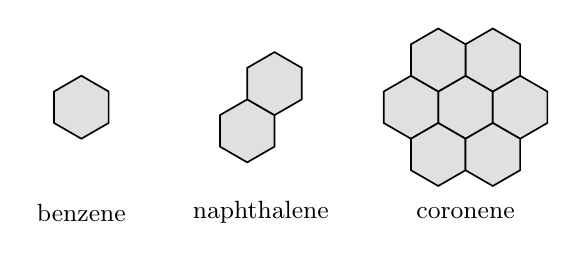
\begin{tikzpicture}[scale=0.40]
  \draw[fill=black!12,draw=black,line width=0.6pt] (0.000,1.000) -- (-0.866,0.500) -- (-0.866,-0.500) -- (-0.000,-1.000) -- (0.866,-0.500) -- (0.866,0.500) -- cycle;
  \node[font=\small] at (0.000,-3.350) {benzene};
  \draw[fill=black!12,draw=black,line width=0.6pt] (5.267,0.250) -- (4.401,-0.250) -- (4.401,-1.250) -- (5.267,-1.750) -- (6.133,-1.250) -- (6.133,-0.250) -- cycle;
  \draw[fill=black!12,draw=black,line width=0.6pt] (6.133,1.750) -- (5.267,1.250) -- (5.267,0.250) -- (6.133,-0.250) -- (6.999,0.250) -- (6.999,1.250) -- cycle;
  \node[font=\small] at (5.700,-3.350) {naphthalene};
  \draw[fill=black!12,draw=black,line width=0.6pt] (12.198,1.000) -- (11.332,0.500) -- (11.332,-0.500) -- (12.198,-1.000) -- (13.064,-0.500) -- (13.064,0.500) -- cycle;
  \draw[fill=black!12,draw=black,line width=0.6pt] (13.930,1.000) -- (13.064,0.500) -- (13.064,-0.500) -- (13.930,-1.000) -- (14.796,-0.500) -- (14.796,0.500) -- cycle;
  \draw[fill=black!12,draw=black,line width=0.6pt] (10.466,1.000) -- (9.600,0.500) -- (9.600,-0.500) -- (10.466,-1.000) -- (11.332,-0.500) -- (11.332,0.500) -- cycle;
  \draw[fill=black!12,draw=black,line width=0.6pt] (13.064,2.500) -- (12.198,2.000) -- (12.198,1.000) -- (13.064,0.500) -- (13.930,1.000) -- (13.930,2.000) -- cycle;
  \draw[fill=black!12,draw=black,line width=0.6pt] (11.332,-0.500) -- (10.466,-1.000) -- (10.466,-2.000) -- (11.332,-2.500) -- (12.198,-2.000) -- (12.198,-1.000) -- cycle;
  \draw[fill=black!12,draw=black,line width=0.6pt] (13.064,-0.500) -- (12.198,-1.000) -- (12.198,-2.000) -- (13.064,-2.500) -- (13.930,-2.000) -- (13.930,-1.000) -- cycle;
  \draw[fill=black!12,draw=black,line width=0.6pt] (11.332,2.500) -- (10.466,2.000) -- (10.466,1.000) -- (11.332,0.500) -- (12.198,1.000) -- (12.198,2.000) -- cycle;
  \node[font=\small] at (12.198,-3.350) {coronene};
\end{tikzpicture}
\caption{Three benzenoids, drawn as sets of cells of the hexagonal tiling.
The graph is the union of the boundary cycles of the chosen cells; the
hydrogen atoms are suppressed, so benzene is a $6$-cycle, naphthalene has
ten vertices and coronene twenty-four.  Six of coronene's vertices lie on
three cells, and benzene and naphthalene have no such vertex; this
distinction is the one that matters, and we will return to it in
Section~\ref{sec:polyhexes}.}
\label{fig:three}
\end{figure}

In H\"uckel molecular orbital theory \cite{Huckel1931,CDS1995,GutPol1986},
the energy levels of the $\pi$-electrons of a conjugated hydrocarbon are, up
to an affine change of units, the eigenvalues of the adjacency matrix of its
carbon skeleton.  A skeleton on $n$ vertices carries $n$ such electrons, and
they occupy the $n/2$ largest eigenvalues, which are the $n/2$ lowest
energies.  Writing the eigenvalues as
$\lambda_1\ge\cdots\ge\lambda_n$, the highest occupied molecular orbital
corresponds to $\lambda_{n/2}$ and the lowest unoccupied one to
$\lambda_{n/2+1}$, and their difference is the \textsl{HOMO--LUMO gap}, a
basic index of kinetic stability.  Mohar \cite{Mohar2015} proposed the study
of these \textsl{median eigenvalues} as a problem in spectral graph theory in
its own right, and showed in \cite{Mohar2016} that the median eigenvalues
of a connected bipartite subcubic graph other than the Heawood graph lie in
$[-1,1]$;
see also \cite{MohTay2015,GuoMoh2014}.
For a bipartite graph, the pairing theorem of Coulson and Rushbrooke
\cite{CouRus1940} says that the spectrum is symmetric about $0$, so
$\lambda_{n/2+1}=-\lambda_{n/2}$ and the HOMO--LUMO gap is $2\lambda_{n/2}$.
The whole question is how close the innermost pair of eigenvalues comes to
zero.

Which graphs keep an interval around zero free of eigenvalues is a spectral
gap problem.  Koll\'ar and Sarnak \cite{KolSar2021} studied the intervals
avoided by the spectra of all, or of infinitely many, cubic graphs, and the
cubic graphs with no eigenvalue in $(-1,1)$ and those with no eigenvalue in
$(-2,0)$ were characterized in \cite{GuoRoy2024,GuoRoy2025}; each of these
two intervals is avoided by infinitely many cubic graphs.  The question we
answer here is of the same kind, for polyhexes and the interval
$(-\thetaG,\thetaG)$, and the answer is finite.

Fowler and Pisanski \cite{FowPis2010} plotted the median eigenvalues of all
connected graphs with maximum degree at most three on at most twelve vertices,
and observed a conspicuous line of graphs with $\lambda_{n/2}=1/\vphi$
exactly, where $\vphi=(1+\sqrt5)/2$ is the golden ratio.  Just over one
percent of these graphs lie on the line, and they wrote that it is not clear
why one eigenvalue should stand out in this way.  Pisanski \cite{Pis2010}
called a graph \textsl{golden} when its median eigenvalues are exactly
$\pm1/\vphi$, listed the small golden graphs and the known golden fullerenes,
amongst them the truncated icosahedron $\mathrm{C}_{60}$
\cite{FowPis2010b}, and asked whether naphthalene is the only golden
benzenoid.  In this paper we show that it is.

We will write
\[
 \vphi=\frac{1+\sqrt5}{2},\qquad
 \thetaG=\vphi\inv=\vphi-1=\frac{\sqrt5-1}{2},
\]
so $\vphi\approx1.618034$ and $\thetaG\approx0.618034$.  Rather than asking
which benzenoids attain $\thetaG$, we ask which ones keep the open interval
$(-\thetaG,\thetaG)$ free of eigenvalues.  This is a formally stronger
question, and its answer is the main result of the paper.  We will state it
for polyhexes, which are the connected unions of hexagons with holes
permitted; benzenoids are the polyhexes without holes, so the result applies
to them a fortiori.  All terms are defined in Section~\ref{sec:polyhexes}.

\begin{theorem}[golden gap theorem]\label{thm:gap}
Let $H$ be a polyhex.  Then $X(H)$ has no eigenvalue in the open interval
$(-\thetaG,\thetaG)$ if and only if $H$ is benzene, naphthalene or
triphenylene.
\end{theorem}

The smallest positive eigenvalues of benzene, naphthalene and triphenylene
are $1$, $\thetaG$ and approximately $0.684040$.  Only naphthalene attains
$\thetaG$, and we obtain the answer to Pisanski's question.

\begin{corollary}\label{cor:pisanski}
Naphthalene is the only golden benzenoid.  More generally, it is the only
polyhex of even order whose median eigenvalues are $\pm\thetaG$.
\end{corollary}

Median eigenvalues are defined only for graphs of even order, and the
restriction costs nothing: a polyhex of odd order has colour classes of
different sizes, so $0$ is an eigenvalue of its graph and it lies outside the
golden gap class.

The proof of Theorem~\ref{thm:gap} has two parts.  Polyhexes with at most
six hexagons are finite in number and are checked directly.  For the rest we
prove a locality theorem, which says that the failure to avoid
$(-\thetaG,\thetaG)$ is always visible inside seven hexagons.  To state it we
need one piece of notation.  For a set $C$ of hexagons of a polyhex $H$ with
graph $X$ and adjacency matrix $A$, let $V(C)$ be the set of vertices lying
on the hexagons of $C$, and let $M_C(H)$ be the principal submatrix of
$A^2-\thetaG^2I$ whose rows and columns are indexed by $V(C)$.  We will see
in Section~\ref{sec:spectral} that $X$ avoids $(-\thetaG,\thetaG)$ if and
only if $A^2-\thetaG^2I$ is positive semidefinite, and that positive
semidefiniteness is inherited by principal submatrices.  Thus a single set
$C$ with $M_C(H)$ not positive semidefinite shows that $X$ has an eigenvalue
in $(-\thetaG,\thetaG)$; we will call such a set an obstruction.  Cells of the
tiling carry the coordinates fixed in Section~\ref{sec:polyhexes} and are
ordered lexicographically there.  A translation of the tiling does not change
the graph of a polyhex, so we may translate $H$ so that its lexicographically
first hexagon is the origin, and the seven hexagons we find can then be taken
to include it.

\begin{theorem}[seven-hexagon theorem]\label{thm:seven}
Let $H$ be a polyhex with at least seven hexagons, translated so that its
lexicographically first hexagon is the origin.  Then $H$ contains a connected
set $C$ of exactly seven hexagons with $(0,0)\in C$ such that $M_C(H)$ is not
positive semidefinite.
\end{theorem}

In particular, every polyhex with at least seven hexagons contains a connected
seven-hexagon obstruction.  The rooted form is the one the proof produces and
the one the cross-checks of Section~\ref{sec:verification} test, and it turns
the theorem into a search of bounded size around a single hexagon.

Seven cannot be replaced by six: we will exhibit a ten-hexagon benzenoid,
not in the class of Theorem~\ref{thm:gap}, in which every connected set of at
most six hexagons has a positive semidefinite block
(Proposition~\ref{prop:nosix} and Corollary~\ref{cor:nosix}).

The proof of Theorem~\ref{thm:seven} is computer-assisted.  The difficulty
is that $M_C(H)$ depends not only on $C$ but on the hexagons of $H$
surrounding $C$, so the finite objects of the proof are not the $333$
heptahexes, the connected sets of seven cells up to the symmetries of the
tiling, but seven-hexagon cores decorated with partial information about
their surroundings.  We have made an effort to make the computation
checkable.  After a rooting reduction, the set of configurations that need
to be examined is finite and explicit, and the proof is a certificate
consisting of $3{,}652$ rooted cores, $22{,}009$ decorated patterns, each
carrying an integer witness, and a covering directed acyclic graph with
$345{,}554$ nodes.  Every spectral claim in the certificate is a strict
inequality between integers, and the test is exact and not a relaxation, so
no floating-point or algebraic-number comparison occurs on the decision path.
The same is true of the other half of the proof of Theorem~\ref{thm:gap}, the
$116$ polyhexes with at most six hexagons: $113$ of them carry an integer
witness decided by the same comparison, and the remaining three are benzene,
naphthalene and triphenylene, whose characteristic polynomials are
classical.  The certificate has been checked by two independently written
verifiers, and the resulting theorem has been cross-checked against exact
spectra for all polyhexes with at most nine hexagons.
Section~\ref{sec:verification} describes what was checked and what the
computation does not establish.

The proof uses none of the structure theory of benzenoids.  It does not use
simple connectivity, Kekul\'e structures, the count of internal vertices, or
the distinction between catacondensed and pericondensed systems.  It is: a
spectral reduction (Section~\ref{sec:spectral}), an explanation of why seven
hexagons and their surroundings are the right objects together with the proof
that seven is best possible (Section~\ref{sec:why}), the seven-hexagon theorem
(Section~\ref{sec:seven}), and the small cases
(Section~\ref{sec:small}).

\section{Polyhexes and benzenoids}\label{sec:polyhexes}

The purpose of this section is to fix terminology; we defer to
Gutman and Cyvin \cite{GutCyv1989} for the theory of benzenoid systems and
to Godsil and Royle \cite{GodRoy2001} for graph-theoretic background.

Fix the infinite hexagonal tiling of the plane.  Its bounded faces are
\textsl{cells}; the chemical literature calls them \textsl{hexagons} or
\textsl{rings}, and we will use the three words interchangeably.  Every
vertex of the tiling lies on exactly three cells, and each two of these three
cells share an edge; thus two cells that share a vertex share an edge.  Two
distinct cells therefore either share exactly one edge, in which case we call
them \textsl{adjacent}, or they are disjoint.  A finite set of cells has a
connected union if and only if the graph on the set whose edges are the
adjacent pairs is connected.  We will call this graph the \textsl{cell
adjacency graph} of the set.

A \textsl{polyhex} is a finite nonempty set $H$ of cells whose union is
connected.  Its \textsl{graph} $X(H)$ has as vertices the vertices of the
tiling lying on cells of $H$, and as edges the edges of the tiling lying on
cells of $H$; in other words, $X(H)$ is the union of the boundary cycles of
the cells of $H$.  The graph $X(H)$ has cycles of length six of its own; we
reserve the word \textsl{cycle} for cycles of $X(H)$ and never call them
hexagons.  We will write $h=\abs H$ for the number of cells.  A
\textsl{benzenoid} is a polyhex whose union is simply connected, that is,
whose union has no holes; a polyhex with holes is called a
\textsl{coronoid} \cite{CyvBruCyv1991}.  The smallest coronoid is the ring of
six cells surrounding an empty cell, with $h=6$.  We will not need the
distinction, since our results hold for all polyhexes.  There are
$1,1,3,7,22,81,331,1435,6505$ benzenoids with $h=1,\ldots,9$ cells
\cite{BriCapHan2002}, and $1,1,3,7,22,82,333,1448,6572$ polyhexes
\cite{OEIS}, counted up to the symmetries of the tiling.

The graph $X(H)$ is planar, and since the tiling is bipartite, so is $X(H)$.
Every vertex of $X(H)$ lies on one, two or three cells of $H$; a vertex on
one cell has degree $2$, and a vertex on two or three cells has degree $3$.
A vertex lying on three cells of $H$ is an \textsl{internal vertex}.  A
benzenoid is \textsl{catacondensed} if it has no internal vertices and
\textsl{pericondensed} otherwise.  The cell adjacency graph of a
catacondensed benzenoid is a tree, and a catacondensed benzenoid has $4h+2$
vertices; in general a benzenoid with $n_i$ internal vertices has $4h+2-n_i$
vertices \cite{GutCyv1989}.  Every cycle of $X(H)$ has length at least six.  In
particular, $X(H)$ has no cycle of length four, and so two distinct vertices
of $X(H)$ have at most one common neighbour.

Figure~\ref{fig:small} shows five small benzenoids.  Anthracene and
phenanthrene both have three cells and $14$ vertices, and differ only in
whether the third cell is attached in line with the first two or at an angle.
That difference already changes the spectrum: their smallest positive
eigenvalues are approximately $0.4142$ and $0.6052$.

\begin{figure}[ht]
\centering
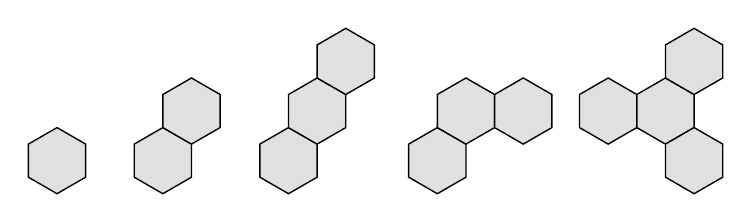
\begin{tikzpicture}[scale=0.42]
\begin{scope}[shift={(0.00,0)}]
  \draw[fill=black!12,draw=black,line width=0.5pt] (0.000,1.000) -- (-0.866,0.500) -- (-0.866,-0.500) -- (-0.000,-1.000) -- (0.866,-0.500) -- (0.866,0.500) -- cycle;
\end{scope}
\begin{scope}[shift={(3.20,0)}]
  \draw[fill=black!12,draw=black,line width=0.5pt] (0.000,1.000) -- (-0.866,0.500) -- (-0.866,-0.500) -- (-0.000,-1.000) -- (0.866,-0.500) -- (0.866,0.500) -- cycle;
  \draw[fill=black!12,draw=black,line width=0.5pt] (0.866,2.500) -- (-0.000,2.000) -- (0.000,1.000) -- (0.866,0.500) -- (1.732,1.000) -- (1.732,2.000) -- cycle;
\end{scope}
\begin{scope}[shift={(7.00,0)}]
  \draw[fill=black!12,draw=black,line width=0.5pt] (0.000,1.000) -- (-0.866,0.500) -- (-0.866,-0.500) -- (-0.000,-1.000) -- (0.866,-0.500) -- (0.866,0.500) -- cycle;
  \draw[fill=black!12,draw=black,line width=0.5pt] (0.866,2.500) -- (-0.000,2.000) -- (0.000,1.000) -- (0.866,0.500) -- (1.732,1.000) -- (1.732,2.000) -- cycle;
  \draw[fill=black!12,draw=black,line width=0.5pt] (1.732,4.000) -- (0.866,3.500) -- (0.866,2.500) -- (1.732,2.000) -- (2.598,2.500) -- (2.598,3.500) -- cycle;
\end{scope}
\begin{scope}[shift={(11.50,0)}]
  \draw[fill=black!12,draw=black,line width=0.5pt] (0.000,1.000) -- (-0.866,0.500) -- (-0.866,-0.500) -- (-0.000,-1.000) -- (0.866,-0.500) -- (0.866,0.500) -- cycle;
  \draw[fill=black!12,draw=black,line width=0.5pt] (0.866,2.500) -- (-0.000,2.000) -- (0.000,1.000) -- (0.866,0.500) -- (1.732,1.000) -- (1.732,2.000) -- cycle;
  \draw[fill=black!12,draw=black,line width=0.5pt] (2.598,2.500) -- (1.732,2.000) -- (1.732,1.000) -- (2.598,0.500) -- (3.464,1.000) -- (3.464,2.000) -- cycle;
\end{scope}
\begin{scope}[shift={(15.80,0)}]
  \draw[fill=black!12,draw=black,line width=0.5pt] (0.866,2.500) -- (-0.000,2.000) -- (0.000,1.000) -- (0.866,0.500) -- (1.732,1.000) -- (1.732,2.000) -- cycle;
  \draw[fill=black!12,draw=black,line width=0.5pt] (2.598,2.500) -- (1.732,2.000) -- (1.732,1.000) -- (2.598,0.500) -- (3.464,1.000) -- (3.464,2.000) -- cycle;
  \draw[fill=black!12,draw=black,line width=0.5pt] (3.464,4.000) -- (2.598,3.500) -- (2.598,2.500) -- (3.464,2.000) -- (4.330,2.500) -- (4.330,3.500) -- cycle;
  \draw[fill=black!12,draw=black,line width=0.5pt] (3.464,1.000) -- (2.598,0.500) -- (2.598,-0.500) -- (3.464,-1.000) -- (4.330,-0.500) -- (4.330,0.500) -- cycle;
\end{scope}
\end{tikzpicture}
\caption{From left to right: benzene, naphthalene, anthracene, phenanthrene
and triphenylene, drawn as sets of cells of the hexagonal tiling.  Their
smallest positive eigenvalues are $1$, $\thetaG\approx0.6180$, $0.4142$,
$0.6052$ and $0.6840$.  The first two and the last are the members of the
golden gap class.}
\label{fig:small}
\end{figure}

We will need coordinates for cells.  Use \textsl{axial coordinates}, in
which the cells of the tiling are the pairs $(q,r)\in\ints^2$, and two cells
are adjacent when they differ by one of the six vectors
\[
 (1,0),\quad(-1,0),\quad(0,1),\quad(0,-1),\quad(1,-1),\quad(-1,1).
\]
The distance between cells in the cell adjacency graph of the whole tiling is
then
\[
 d\bigl((q,r),(q',r')\bigr)
 =\max\bigl\{\abs{q-q'},\,\abs{r-r'},\,\abs{(q+r)-(q'+r')}\bigr\},
\]
and we write $d(q,r)$ for the distance from $(q,r)$ to the origin.  We order
cells lexicographically by $(q,r)$.  A translation of the tiling carries
polyhexes to polyhexes with isomorphic graphs, so we may always translate a
polyhex so that its lexicographically first cell is the origin.

\section{Spectra and the golden gap}\label{sec:spectral}

Let $X$ be a graph with vertex set $V$.  The \textsl{adjacency matrix} $A=A(X)$
is the symmetric $01$-matrix with rows and columns indexed by $V$ whose
$(u,v)$-entry is $1$ if and only if $u$ and $v$ are adjacent.  We will use
functional notation for the entries of matrices and vectors; the $uv$-entry
of a matrix $M$ is written $M(u,v)$, and the entry of a vector $\Zy$ indexed
by $u$ is written $\Zy(u)$.  The \textsl{spectrum} $\spec X$ of $X$ is the
multiset of eigenvalues of $A$, which are real since $A$ is symmetric, and
we will call these the \textsl{eigenvalues of $X$}.  Order them
$\lambda_1\ge\lambda_2\ge\cdots\ge\lambda_n$, where $n=\abs V$.  When $n$ is
even, the \textsl{median eigenvalues} of $X$ are $\lambda_{n/2}$ and
$\lambda_{n/2+1}$, and the \textsl{HOMO--LUMO gap} is their difference.

If $X$ is bipartite, then $\lambda$ and $-\lambda$ are eigenvalues of $X$
with the same multiplicity, for every real $\lambda$; this is the pairing
theorem of Coulson and Rushbrooke \cite{CouRus1940}.
Thus for a bipartite graph on an even number $n$ of vertices the median
eigenvalues are $\pm\lambda_{n/2}$, and they are $\pm\thetaG$ exactly when
$\lambda_{n/2}=\thetaG$.  Following Pisanski \cite{Pis2010}, we will say that
a bipartite graph on an even number of vertices is \textsl{golden} if its
median eigenvalues are
$\pm\thetaG$.  We use the word in Pisanski's sense throughout; Estrada
\cite{Est2007} uses the same phrase for a different class of graphs, defined
by a condition on a ratio of spectral quantities, and Pisanski's
disambiguating name for the graphs considered here is \textsl{golden
HOMO--LUMO graph}.  A bipartite graph whose two colour classes have different
sizes has $0$ as an eigenvalue, with multiplicity at least the difference of
the sizes, and so is not golden.

We will say that a polyhex $H$ lies in the \textsl{golden gap class} if
$X(H)$ has no eigenvalue in the open interval $(-\thetaG,\thetaG)$.  A golden
polyhex lies in the golden gap class, since its eigenvalues other than the
median pair have absolute value at least $\thetaG$ by the
pairing theorem.  Conversely, a member of the golden gap class has no
eigenvalue $0$, so its order $n$ is even, exactly $n/2$ of its eigenvalues are
positive, and $\lambda_{n/2}$ is the smallest of these; and so it is golden
if and only if $\thetaG$ is one of its eigenvalues.  Thus
Corollary~\ref{cor:pisanski} follows from Theorem~\ref{thm:gap} once we know
the spectra of the three graphs in Figure~\ref{fig:small}; benzene is the
$6$-cycle, with spectrum $\pm2,\pm1,\pm1$, naphthalene has $\thetaG$ as a
simple eigenvalue, and the smallest positive eigenvalue of triphenylene is
the root $0.684040\ldots$ of $x^{6}-6x^{4}+9x^{2}-3$, a factor of its
characteristic polynomial; these are readily computed.

\subsection{Positive semidefiniteness}

A real symmetric matrix $M$ indexed by a set $V$ is \textsl{positive
semidefinite}, written $M\succeq0$, if $\Zy\tp M\Zy\ge0$ for every real
vector $\Zy$ indexed by $V$; equivalently, if every eigenvalue of $M$ is
nonnegative.  For a subset $U\sbs V$, the \textsl{principal submatrix} $M[U]$
is the matrix obtained from $M$ by keeping the rows and columns indexed by
$U$.  If $\Zy$ is a vector indexed by $U$ and $\widetilde{\Zy}$ is its
extension by zero to $V$, then $\Zy\tp M[U]\Zy=\widetilde{\Zy}\tp M
\widetilde{\Zy}$.  We obtain the following two facts, which we will use
repeatedly and without further comment.

\begin{lemma}\label{lem:principal}
Let $M$ be a real symmetric matrix indexed by $V$ and let $U\sbs V$.
\begin{enumerate}
\item[\textup{(a)}] If $M\succeq0$ then $M[U]\succeq0$.
\item[\textup{(b)}] If there is a vector $\Zy$ indexed by $U$ with
 $\Zy\tp M[U]\Zy<0$, then $M\not\succeq0$.  \qed
\end{enumerate}
\end{lemma}

We will call a vector $\Zy$ as in (b) a \textsl{witness} that $M$ is not
positive semidefinite.  The proof of Theorem~\ref{thm:seven} consists
entirely of producing witnesses; the small cases of
Section~\ref{sec:small} require the opposite, a certificate of positive
semidefiniteness.

\subsection{The spectral reduction}

Since the eigenvalues of $A^2$ are the squares of the eigenvalues of $A$, the
golden gap condition is a positive semidefiniteness condition.

\begin{lemma}\label{lem:reduction}
Let $X$ be a graph with adjacency matrix $A$.  Then $X$ has no eigenvalue in
$(-\thetaG,\thetaG)$ if and only if
\[
 A^{2}-\thetaG^{2}I\succeq0 .
\]
If $X$ is bipartite with colour classes $S$ and $T$, and $R$ is the
submatrix of $A$ with rows indexed by $S$ and columns indexed by $T$, then
this holds if and only if
\[
 RR\tp-\thetaG^{2}I\succeq0
 \qquad\text{and}\qquad
 R\tp R-\thetaG^{2}I\succeq0 .
\]
\end{lemma}

\begin{proof}
The eigenvalues of $A^2-\thetaG^2I$ are the numbers $\lambda^2-\thetaG^2$
for $\lambda\in\spec X$, and $\lambda^2\ge\thetaG^2$ if and only if
$\abs\lambda\ge\thetaG$.  If $X$ is bipartite then, ordering the vertices of
$S$ before those of $T$,
\[
 A=\pmat{0 & R\\ R\tp & 0},\qquad
 A^{2}=\pmat{RR\tp & 0\\ 0 & R\tp R},
\]
and a block diagonal matrix is positive semidefinite if and only if each
block is.
\end{proof}

The matrix $R$ is the \textsl{biadjacency matrix} of $X$, and the positive
eigenvalues of $X$ are the singular values of $R$; when $\abs S\ne\abs T$
the matrix $R$ is not square and $0$ is an eigenvalue of $X$, as noted
above.

The entries of $A^2$ are explicit: $A^2(u,u)$ is the degree of $u$, and for
$u\ne v$ the entry $A^2(u,v)$ is the number of common neighbours of $u$ and
$v$.  For the graph of a polyhex, the degrees are $2$ or $3$ and the number
of common neighbours is $0$ or $1$, as we saw in
Section~\ref{sec:polyhexes}.  The following reformulation is not needed for
the proof but explains where the golden ratio comes from.  Since
$\thetaG^2=\thetaG\cdot\thetaG=(\vphi-1)^2=\vphi^2-2\vphi+1=2-\vphi$, we have
$2-\thetaG^2=\vphi$.

\begin{proposition}\label{prop:triangular}
Let $H$ be a polyhex with graph $X$ and colour classes $S$ and $T$.  Let $\Gamma_S$
be the graph on $S$ in which two vertices are adjacent when they have a
common neighbour in $X$, and let $D_S$ be the diagonal $01$-matrix indexed by
$S$ with $D_S(u,u)=1$ exactly when $u$ has degree $3$.  We will call $D_S$ the
\textsl{charge} on $S$, and we will say that a vertex is \textsl{charged} when
it has degree three in $X$.  Then
\[
 RR\tp-\thetaG^{2}I=A(\Gamma_S)+D_S+\vphi I ,
\]
and $H$ lies in the golden gap class if and only if the least eigenvalue of
$A(\Gamma_S)+D_S$ and that of $A(\Gamma_T)+D_T$ are both at least $-\vphi$.
\end{proposition}

\begin{proof}
By the description of the entries of $A^2$, we have $RR\tp=2I+D_S+A(\Gamma_S)$,
and $2-\thetaG^2=\vphi$.  The second statement is Lemma~\ref{lem:reduction}.
\end{proof}

One colour class of the tiling is a triangular lattice, in which two vertices
are adjacent when they have a common neighbour in the tiling.  The graph
$\Gamma_S$ is a subgraph of this lattice; it spans the subgraph induced on $S$, but
in general it is a proper subgraph of that induced subgraph, since the common
neighbour in the tiling of two adjacent vertices of $S$ need not be a vertex
of $X$ at all.  We will call a pair $(Y,D)$, consisting of a subgraph $Y$ of
the triangular lattice and a diagonal $01$-matrix $D$ indexed by the vertices
of $Y$, a \textsl{charged subgraph} of the lattice, and we will call the
least eigenvalue of $A(Y)+D$ the least eigenvalue of the pair.  Thus
Proposition~\ref{prop:triangular} says that the golden gap class consists of
those polyhexes for which two charged subgraphs of the triangular lattice
have least eigenvalue at least $-\vphi$.  For naphthalene, the least
eigenvalue is exactly $-\vphi$; naphthalene is the equality case.

\subsection{Local blocks}

Let $H$ be a polyhex with graph $X$ and adjacency matrix $A$.  For a set $C$
of cells of $H$, we write $V(C)$ for the set of vertices of $X$ lying on the
cells of $C$, and we define
\begin{equation}\label{eq:MC}
 M_C(H):=\bigl(A^{2}-\thetaG^{2}I\bigr)[V(C)] .
\end{equation}
Since $X$ is bipartite, $A^{2}$ has no nonzero entry between the two colour
classes, so every principal submatrix of $A^{2}-\thetaG^{2}I$ is block
diagonal, with one block for the vertices of each colour class in its index
set.  We will call the two blocks of $M_C(H)$ its \textsl{colour blocks}; the
matrix $M_C(H)$ is positive semidefinite if and only if both of its colour
blocks are.
We will say that $C$ is an \textsl{obstruction} in $H$ if
$M_C(H)\not\succeq0$.  By Lemmas~\ref{lem:principal} and
\ref{lem:reduction}, a polyhex containing an obstruction has an eigenvalue in
$(-\thetaG,\thetaG)$.  Note that $M_C(H)$ depends on all of $H$ and not only
on $C$, since the degrees of the vertices of $V(C)$ and their common
neighbours are counted in $X(H)$.  Note also that if $C'\sbs C$ then
$M_{C'}(H)$ is a principal submatrix of $M_C(H)$, so if $C$ is not an
obstruction then neither is any subset of $C$.

The dependence of $M_C(H)$ on $H$ reaches no further than one ring of cells
around $C$.  The \textsl{collar} of $C$ is the set of cells of the tiling
that are not in $C$ and are adjacent to a cell of $C$.  The collar is a set
of cells of the tiling, not of $H$; some of its cells may lie in $H$ and some
may not.

\begin{lemma}\label{lem:collar}
Let $C$ be a set of cells of a polyhex $H$.  Then $M_C(H)$ is determined by
$C$ together with the set of cells of the collar of $C$ that lie in $H$.
\end{lemma}

\begin{proof}
The entries of $M_C(H)$ are the degrees of the vertices in $V(C)$ and the
numbers of common neighbours of pairs of vertices in $V(C)$, and these are
determined by the set of edges of $X(H)$ incident with $V(C)$.  Every such
edge lies on a cell of $H$ containing a vertex $v\in V(C)$.  Let $c$ be such
a cell and suppose $c\notin C$.  Choose $c'\in C$ with $v$ on $c'$.  Exactly
three cells of the tiling contain $v$, and they are pairwise adjacent; since
$c$ and $c'$ are two of them, $c$ is adjacent to $c'$ and so lies in the
collar of $C$.
\end{proof}

\section{Why the collar, and why seven}\label{sec:why}

This section contains the motivation for the objects that the proof of
Theorem~\ref{thm:seven} works with, and the proof that seven is best
possible.

\subsection{The block depends on the surroundings}

Let $C$ be a set of cells of a polyhex $H$.  By Lemma~\ref{lem:collar}, the
block $M_C(H)$ is determined by $C$ together with the cells of the collar of
$C$ that lie in $H$, and it does in general depend on those cells.
Cells of $H$ in the collar raise degrees and create common neighbours, and
they may also add edges between vertices of $V(C)$.  A set of cells that is
an obstruction in isolation need not remain one once it is embedded in a
larger polyhex.  This is not a theoretical worry.

\begin{example}\label{ex:coronene}
Let $C$ be the seven cells of coronene, a central cell with its six
neighbours, and let $H=C$.  Then each of the two colour blocks of $M_C(H)$
has least eigenvalue approximately
$-0.0912$, so $C$ is an obstruction in coronene.  Now let $H$ be
circumcoronene, which consists of $C$ together with all twelve cells of its
collar.  Each colour block of $M_C(H)$ now has least eigenvalue approximately
$+0.4100$; the block is positive definite, and $C$ is not an obstruction in
circumcoronene.  (The two blocks have the same spectrum because a rotation of
the tiling by $60^\circ$ about the central cell exchanges the two colour
classes.)  Circumcoronene is not in the golden gap class, since it has
$54$ vertices and its smallest positive eigenvalue is approximately $0.3420$;
the obstruction is simply elsewhere.
\end{example}

Thus listing the $333$ heptahexes is not enough.  The finite objects in the proof
of Theorem~\ref{thm:seven} are \textsl{decorated} sets of seven cells: a
connected set $C$ of seven cells, a partial assignment of the cells of its
collar as present or absent, and a witness whose negativity survives every
way of completing the assignment.  We will make this precise in
Section~\ref{sec:seven}.

\subsection{Seven is best possible}\label{sec:optimality}

Theorem~\ref{thm:seven} uses seven cells, and seven is the least number for
which such a statement is true.  If a polyhex $H$ is not in the golden gap
class then the set of all of its cells is an obstruction; let $k(H)$ be the
least $k$ such that some connected set of $k$ cells of $H$ is an
obstruction.  Two small benzenoids settle all of $k=1,\ldots,6$ between
them.  (For small $k$ there is nothing to do: a polyhex in the golden gap
class has no obstruction at all, so triphenylene already rules out $k\le4$.)

\begin{proposition}[seven is best possible]\label{prop:nosix}
Let $H_{10}$ be the benzenoid with cells
\[
 (0,3),\ (1,1),\ (1,2),\ (1,4),\ (2,2),\ (2,3),\ (3,0),\ (3,1),\ (3,3),\ (4,1)
\]
and let $H_{7}$ be the benzenoid with cells
\[
 (0,0),\ (0,3),\ (1,0),\ (1,1),\ (1,2),\ (2,-1),\ (2,2) ,
\]
shown on the left and on the right of Figure~\ref{fig:witnesses}.  Neither
lies in the golden gap class, and
\[
 k(H_{10})=7,\qquad k(H_{7})=6 .
\]
\end{proposition}

\begin{proof}
The benzenoid $H_{10}$ is catacondensed, with $42$ vertices, and its
smallest positive eigenvalue is $0.5311319792\ldots<\thetaG$; thus it is not
in the golden gap class.  It has
\[
 10,\quad 9,\quad 12,\quad 16,\quad 24,\quad 27
\]
connected sets of cells of sizes $1,\ldots,6$, and symmetric Gaussian
elimination, pivoting on positive diagonal entries and carried out exactly
over $\rats(\sqrt5)$ as described in Section~\ref{sec:small}, shows that
every one of these sets $C$ has $M_C(H_{10})\succeq0$.  Of the $23$ connected
sets of seven cells, $21$ are obstructions, and so $k(H_{10})=7$.

The benzenoid $H_{7}$ is catacondensed as well.  It has six connected sets of
five cells, none of which is an obstruction, while all four of its connected
sets of six cells are.  Since $H_{7}$ is connected and has seven cells, every
connected set of at most four of its cells extends to a connected set of five
cells; a subset of a set that is not an obstruction is not an obstruction, so
no connected set of at most five cells of $H_{7}$ is an obstruction and
$k(H_{7})=6$.  In particular $H_{7}$ contains an obstruction, so it is not in
the golden gap class either.
\end{proof}

\begin{corollary}\label{cor:nosix}
For no $k\le6$ does every polyhex with at least $k$ cells contain a connected
set of $k$ cells that is an obstruction.
\end{corollary}

\begin{proof}
Let $k\le6$.  If $k=6$, then $H_{10}$ has at least $k$ cells and, since
$k(H_{10})=7$, no connected set of $k$ cells of $H_{10}$ is an obstruction.
If $k\le5$, then $H_{7}$ has at least $k$ cells and, since $k(H_{7})=6$, no
connected set of $k$ cells of $H_{7}$ is an obstruction.
\end{proof}

\begin{figure}[ht]
\centering
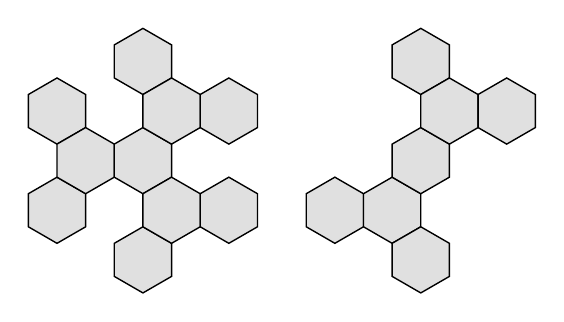
\begin{tikzpicture}[scale=0.42]
\begin{scope}
  \draw[fill=black!12,draw=black,line width=0.5pt] (2.598,5.500) -- (1.732,5.000) -- (1.732,4.000) -- (2.598,3.500) -- (3.464,4.000) -- (3.464,5.000) -- cycle;
  \draw[fill=black!12,draw=black,line width=0.5pt] (2.598,2.500) -- (1.732,2.000) -- (1.732,1.000) -- (2.598,0.500) -- (3.464,1.000) -- (3.464,2.000) -- cycle;
  \draw[fill=black!12,draw=black,line width=0.5pt] (3.464,4.000) -- (2.598,3.500) -- (2.598,2.500) -- (3.464,2.000) -- (4.330,2.500) -- (4.330,3.500) -- cycle;
  \draw[fill=black!12,draw=black,line width=0.5pt] (5.196,7.000) -- (4.330,6.500) -- (4.330,5.500) -- (5.196,5.000) -- (6.062,5.500) -- (6.062,6.500) -- cycle;
  \draw[fill=black!12,draw=black,line width=0.5pt] (5.196,4.000) -- (4.330,3.500) -- (4.330,2.500) -- (5.196,2.000) -- (6.062,2.500) -- (6.062,3.500) -- cycle;
  \draw[fill=black!12,draw=black,line width=0.5pt] (6.062,5.500) -- (5.196,5.000) -- (5.196,4.000) -- (6.062,3.500) -- (6.928,4.000) -- (6.928,5.000) -- cycle;
  \draw[fill=black!12,draw=black,line width=0.5pt] (5.196,1.000) -- (4.330,0.500) -- (4.330,-0.500) -- (5.196,-1.000) -- (6.062,-0.500) -- (6.062,0.500) -- cycle;
  \draw[fill=black!12,draw=black,line width=0.5pt] (6.062,2.500) -- (5.196,2.000) -- (5.196,1.000) -- (6.062,0.500) -- (6.928,1.000) -- (6.928,2.000) -- cycle;
  \draw[fill=black!12,draw=black,line width=0.5pt] (7.794,5.500) -- (6.928,5.000) -- (6.928,4.000) -- (7.794,3.500) -- (8.660,4.000) -- (8.660,5.000) -- cycle;
  \draw[fill=black!12,draw=black,line width=0.5pt] (7.794,2.500) -- (6.928,2.000) -- (6.928,1.000) -- (7.794,0.500) -- (8.660,1.000) -- (8.660,2.000) -- cycle;
\end{scope}
\begin{scope}[shift={(11,1.5)}]
  \draw[fill=black!12,draw=black,line width=0.5pt] (0.000,1.000) -- (-0.866,0.500) -- (-0.866,-0.500) -- (-0.000,-1.000) -- (0.866,-0.500) -- (0.866,0.500) -- cycle;
  \draw[fill=black!12,draw=black,line width=0.5pt] (2.598,5.500) -- (1.732,5.000) -- (1.732,4.000) -- (2.598,3.500) -- (3.464,4.000) -- (3.464,5.000) -- cycle;
  \draw[fill=black!12,draw=black,line width=0.5pt] (1.732,1.000) -- (0.866,0.500) -- (0.866,-0.500) -- (1.732,-1.000) -- (2.598,-0.500) -- (2.598,0.500) -- cycle;
  \draw[fill=black!12,draw=black,line width=0.5pt] (2.598,2.500) -- (1.732,2.000) -- (1.732,1.000) -- (2.598,0.500) -- (3.464,1.000) -- (3.464,2.000) -- cycle;
  \draw[fill=black!12,draw=black,line width=0.5pt] (3.464,4.000) -- (2.598,3.500) -- (2.598,2.500) -- (3.464,2.000) -- (4.330,2.500) -- (4.330,3.500) -- cycle;
  \draw[fill=black!12,draw=black,line width=0.5pt] (2.598,-0.500) -- (1.732,-1.000) -- (1.732,-2.000) -- (2.598,-2.500) -- (3.464,-2.000) -- (3.464,-1.000) -- cycle;
  \draw[fill=black!12,draw=black,line width=0.5pt] (5.196,4.000) -- (4.330,3.500) -- (4.330,2.500) -- (5.196,2.000) -- (6.062,2.500) -- (6.062,3.500) -- cycle;
\end{scope}
\end{tikzpicture}
\caption{The two witnesses of Proposition~\ref{prop:nosix}.  Left: the
catacondensed benzenoid $H_{10}$, in which no connected set of at most six
cells is an obstruction, although $21$ of its $23$ connected seven-cell sets
are.  Right: the seven-cell benzenoid $H_{7}$, in which no connected set of
at most five cells is an obstruction, although all four of its connected
six-cell sets are.}
\label{fig:witnesses}
\end{figure}

The smaller witness already settles $k\le5$, so the ten cells of $H_{10}$ are
needed only for $k=6$.  Note the mechanism.  The obstruction can stay
invisible at scale six even in a benzenoid that is comfortably outside the
golden gap class, so the seven in Theorem~\ref{thm:seven} is a feature of the
problem and not an artefact of the method.

\section{Seven hexagons suffice}\label{sec:seven}

This section proves Theorem~\ref{thm:seven}.  The reduction to a finite
problem is elementary; the finite problem is then discharged by a certificate
whose verification we describe in Section~\ref{sec:verification}.

\subsection{Rooting}\label{sec:rooting}

Let $H$ be a polyhex with at least seven cells, translated so that its
lexicographically first cell is the origin $(0,0)$.  Every cell of $H$ then
lies in the half-plane
\begin{equation}\label{eq:halfplane}
 \Lambda^{+}=\{(q,r):q>0\}\cup\{(0,r):r\ge0\} .
\end{equation}
This is immediate from the definition of the lexicographic order on cells.
We will call a polyhex whose lexicographically first cell is the origin a
\textsl{rooted polyhex}; every rooted polyhex is contained in $\Lambda^{+}$,
and that containment is what the arguments below use.
For $j\ge0$, put $W_j=\{(q,r)\in\Lambda^{+}:d(q,r)\le j\}$.  The map
$(q,r)\mapsto(-q,-r)$ pairs the cells at distance at most $j$ from the
origin, other than the origin itself, and $\Lambda^{+}$ contains exactly one cell
of each pair; since there are $3j^2+3j+1$ cells at distance at most $j$, it
is easy to see that $\abs{W_j}=(3j^2+3j+2)/2$.  In particular
\begin{equation}\label{eq:W-counts}
 \abs{W_6}=64,\qquad\abs{W_7}=85 .
\end{equation}

A \textsl{rooted core} is a connected set of seven cells of $\Lambda^{+}$ that
contains the origin.  Since a rooted core is connected and contains the
origin, each of its cells is within distance six of the origin, so every
rooted core lies in $W_6$.  Expanding connected sets one cell at a time
inside $\Lambda^{+}$, we find that there are exactly
\begin{equation}\label{eq:cores}
 3{,}652
\end{equation}
rooted cores.  This is a rooted count: once the half-plane has been fixed,
no rotation or reflection is factored out.  The polyhex $H$ contains a rooted
core: run a breadth-first search in the cell adjacency graph of $H$ from the
origin and stop when seven cells have been found.

\begin{lemma}\label{lem:local}
Let $H$ be a rooted polyhex and
let $C$ be a rooted core contained in $H$.  Then every cell of the collar of
$C$ that lies in $H$ lies in $W_7$.  Thus $M_C(H)$ is determined by
$C$ and by the set $H\cap W_7$.
\end{lemma}

\begin{proof}
A cell of the collar of $C$ is adjacent to a cell of $C\sbs W_6$, so it is
within distance seven of the origin; if it lies in $H$ then it lies in
$\Lambda^{+}$ by \eqref{eq:halfplane}, and so in $W_7$.  The second statement now
follows from Lemma~\ref{lem:collar}.
\end{proof}

We will write $\collarp(C)$ for the set of cells of the collar of $C$ that lie
in $\Lambda^{+}$, and we will call it the \textsl{admissible collar} of $C$.
By Lemma~\ref{lem:local} these are exactly the collar cells that can lie in a
rooted polyhex, and they lie in $W_7$; a collar cell outside $\Lambda^{+}$ is
absent from every rooted polyhex, and we will treat it throughout as forced
absent.

We will call the set $W_7$ the \textsl{window}, and we will call a subset of
$W_7$ an \textsl{occupancy pattern}.  By
Lemma~\ref{lem:local}, once $H$ is rooted, the block $M_C(H)$ for any rooted
core $C\sbs H$ is a function of the occupancy pattern $H\cap W_7$, an
$85$-bit object.  There are finitely many occupancy patterns, and
Theorem~\ref{thm:seven} has become a finite statement.  Figure~\ref{fig:window}
shows the window with a rooted core and its collar.  The core drawn there is
coronene, a central cell with its six neighbours, placed so that its
lexicographically first cell is the origin; its collar has twelve cells, of
which eight lie in $W_7$ and four lie outside $\Lambda^{+}$ and are therefore
absent from every rooted polyhex.  With all eight permitted collar cells
present, the two colour blocks of $M_C$ have least eigenvalues approximately
$+0.0141$ and $+0.1998$, so this core is not an obstruction in that
configuration, and the cover of Section~\ref{sec:cover} must supply a
different core.

\begin{figure}[ht]
\centering
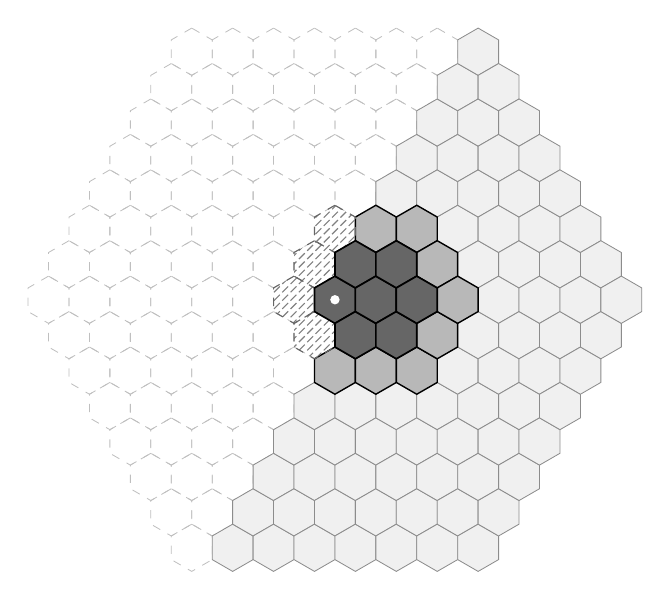
\begin{tikzpicture}[scale=0.30]
  \draw[fill=none,draw=black!25,line width=0.3pt,dashed] (-12.124,1.000) -- (-12.990,0.500) -- (-12.990,-0.500) -- (-12.124,-1.000) -- (-11.258,-0.500) -- (-11.258,0.500) -- cycle;
  \draw[fill=none,draw=black!25,line width=0.3pt,dashed] (-11.258,2.500) -- (-12.124,2.000) -- (-12.124,1.000) -- (-11.258,0.500) -- (-10.392,1.000) -- (-10.392,2.000) -- cycle;
  \draw[fill=none,draw=black!25,line width=0.3pt,dashed] (-10.392,4.000) -- (-11.258,3.500) -- (-11.258,2.500) -- (-10.392,2.000) -- (-9.526,2.500) -- (-9.526,3.500) -- cycle;
  \draw[fill=none,draw=black!25,line width=0.3pt,dashed] (-9.526,5.500) -- (-10.392,5.000) -- (-10.392,4.000) -- (-9.526,3.500) -- (-8.660,4.000) -- (-8.660,5.000) -- cycle;
  \draw[fill=none,draw=black!25,line width=0.3pt,dashed] (-8.660,7.000) -- (-9.526,6.500) -- (-9.526,5.500) -- (-8.660,5.000) -- (-7.794,5.500) -- (-7.794,6.500) -- cycle;
  \draw[fill=none,draw=black!25,line width=0.3pt,dashed] (-7.794,8.500) -- (-8.660,8.000) -- (-8.660,7.000) -- (-7.794,6.500) -- (-6.928,7.000) -- (-6.928,8.000) -- cycle;
  \draw[fill=none,draw=black!25,line width=0.3pt,dashed] (-6.928,10.000) -- (-7.794,9.500) -- (-7.794,8.500) -- (-6.928,8.000) -- (-6.062,8.500) -- (-6.062,9.500) -- cycle;
  \draw[fill=none,draw=black!25,line width=0.3pt,dashed] (-6.062,11.500) -- (-6.928,11.000) -- (-6.928,10.000) -- (-6.062,9.500) -- (-5.196,10.000) -- (-5.196,11.000) -- cycle;
  \draw[fill=none,draw=black!25,line width=0.3pt,dashed] (-11.258,-0.500) -- (-12.124,-1.000) -- (-12.124,-2.000) -- (-11.258,-2.500) -- (-10.392,-2.000) -- (-10.392,-1.000) -- cycle;
  \draw[fill=none,draw=black!25,line width=0.3pt,dashed] (-10.392,1.000) -- (-11.258,0.500) -- (-11.258,-0.500) -- (-10.392,-1.000) -- (-9.526,-0.500) -- (-9.526,0.500) -- cycle;
  \draw[fill=none,draw=black!25,line width=0.3pt,dashed] (-9.526,2.500) -- (-10.392,2.000) -- (-10.392,1.000) -- (-9.526,0.500) -- (-8.660,1.000) -- (-8.660,2.000) -- cycle;
  \draw[fill=none,draw=black!25,line width=0.3pt,dashed] (-8.660,4.000) -- (-9.526,3.500) -- (-9.526,2.500) -- (-8.660,2.000) -- (-7.794,2.500) -- (-7.794,3.500) -- cycle;
  \draw[fill=none,draw=black!25,line width=0.3pt,dashed] (-7.794,5.500) -- (-8.660,5.000) -- (-8.660,4.000) -- (-7.794,3.500) -- (-6.928,4.000) -- (-6.928,5.000) -- cycle;
  \draw[fill=none,draw=black!25,line width=0.3pt,dashed] (-6.928,7.000) -- (-7.794,6.500) -- (-7.794,5.500) -- (-6.928,5.000) -- (-6.062,5.500) -- (-6.062,6.500) -- cycle;
  \draw[fill=none,draw=black!25,line width=0.3pt,dashed] (-6.062,8.500) -- (-6.928,8.000) -- (-6.928,7.000) -- (-6.062,6.500) -- (-5.196,7.000) -- (-5.196,8.000) -- cycle;
  \draw[fill=none,draw=black!25,line width=0.3pt,dashed] (-5.196,10.000) -- (-6.062,9.500) -- (-6.062,8.500) -- (-5.196,8.000) -- (-4.330,8.500) -- (-4.330,9.500) -- cycle;
  \draw[fill=none,draw=black!25,line width=0.3pt,dashed] (-4.330,11.500) -- (-5.196,11.000) -- (-5.196,10.000) -- (-4.330,9.500) -- (-3.464,10.000) -- (-3.464,11.000) -- cycle;
  \draw[fill=none,draw=black!25,line width=0.3pt,dashed] (-10.392,-2.000) -- (-11.258,-2.500) -- (-11.258,-3.500) -- (-10.392,-4.000) -- (-9.526,-3.500) -- (-9.526,-2.500) -- cycle;
  \draw[fill=none,draw=black!25,line width=0.3pt,dashed] (-9.526,-0.500) -- (-10.392,-1.000) -- (-10.392,-2.000) -- (-9.526,-2.500) -- (-8.660,-2.000) -- (-8.660,-1.000) -- cycle;
  \draw[fill=none,draw=black!25,line width=0.3pt,dashed] (-8.660,1.000) -- (-9.526,0.500) -- (-9.526,-0.500) -- (-8.660,-1.000) -- (-7.794,-0.500) -- (-7.794,0.500) -- cycle;
  \draw[fill=none,draw=black!25,line width=0.3pt,dashed] (-7.794,2.500) -- (-8.660,2.000) -- (-8.660,1.000) -- (-7.794,0.500) -- (-6.928,1.000) -- (-6.928,2.000) -- cycle;
  \draw[fill=none,draw=black!25,line width=0.3pt,dashed] (-6.928,4.000) -- (-7.794,3.500) -- (-7.794,2.500) -- (-6.928,2.000) -- (-6.062,2.500) -- (-6.062,3.500) -- cycle;
  \draw[fill=none,draw=black!25,line width=0.3pt,dashed] (-6.062,5.500) -- (-6.928,5.000) -- (-6.928,4.000) -- (-6.062,3.500) -- (-5.196,4.000) -- (-5.196,5.000) -- cycle;
  \draw[fill=none,draw=black!25,line width=0.3pt,dashed] (-5.196,7.000) -- (-6.062,6.500) -- (-6.062,5.500) -- (-5.196,5.000) -- (-4.330,5.500) -- (-4.330,6.500) -- cycle;
  \draw[fill=none,draw=black!25,line width=0.3pt,dashed] (-4.330,8.500) -- (-5.196,8.000) -- (-5.196,7.000) -- (-4.330,6.500) -- (-3.464,7.000) -- (-3.464,8.000) -- cycle;
  \draw[fill=none,draw=black!25,line width=0.3pt,dashed] (-3.464,10.000) -- (-4.330,9.500) -- (-4.330,8.500) -- (-3.464,8.000) -- (-2.598,8.500) -- (-2.598,9.500) -- cycle;
  \draw[fill=none,draw=black!25,line width=0.3pt,dashed] (-2.598,11.500) -- (-3.464,11.000) -- (-3.464,10.000) -- (-2.598,9.500) -- (-1.732,10.000) -- (-1.732,11.000) -- cycle;
  \draw[fill=none,draw=black!25,line width=0.3pt,dashed] (-9.526,-3.500) -- (-10.392,-4.000) -- (-10.392,-5.000) -- (-9.526,-5.500) -- (-8.660,-5.000) -- (-8.660,-4.000) -- cycle;
  \draw[fill=none,draw=black!25,line width=0.3pt,dashed] (-8.660,-2.000) -- (-9.526,-2.500) -- (-9.526,-3.500) -- (-8.660,-4.000) -- (-7.794,-3.500) -- (-7.794,-2.500) -- cycle;
  \draw[fill=none,draw=black!25,line width=0.3pt,dashed] (-7.794,-0.500) -- (-8.660,-1.000) -- (-8.660,-2.000) -- (-7.794,-2.500) -- (-6.928,-2.000) -- (-6.928,-1.000) -- cycle;
  \draw[fill=none,draw=black!25,line width=0.3pt,dashed] (-6.928,1.000) -- (-7.794,0.500) -- (-7.794,-0.500) -- (-6.928,-1.000) -- (-6.062,-0.500) -- (-6.062,0.500) -- cycle;
  \draw[fill=none,draw=black!25,line width=0.3pt,dashed] (-6.062,2.500) -- (-6.928,2.000) -- (-6.928,1.000) -- (-6.062,0.500) -- (-5.196,1.000) -- (-5.196,2.000) -- cycle;
  \draw[fill=none,draw=black!25,line width=0.3pt,dashed] (-5.196,4.000) -- (-6.062,3.500) -- (-6.062,2.500) -- (-5.196,2.000) -- (-4.330,2.500) -- (-4.330,3.500) -- cycle;
  \draw[fill=none,draw=black!25,line width=0.3pt,dashed] (-4.330,5.500) -- (-5.196,5.000) -- (-5.196,4.000) -- (-4.330,3.500) -- (-3.464,4.000) -- (-3.464,5.000) -- cycle;
  \draw[fill=none,draw=black!25,line width=0.3pt,dashed] (-3.464,7.000) -- (-4.330,6.500) -- (-4.330,5.500) -- (-3.464,5.000) -- (-2.598,5.500) -- (-2.598,6.500) -- cycle;
  \draw[fill=none,draw=black!25,line width=0.3pt,dashed] (-2.598,8.500) -- (-3.464,8.000) -- (-3.464,7.000) -- (-2.598,6.500) -- (-1.732,7.000) -- (-1.732,8.000) -- cycle;
  \draw[fill=none,draw=black!25,line width=0.3pt,dashed] (-1.732,10.000) -- (-2.598,9.500) -- (-2.598,8.500) -- (-1.732,8.000) -- (-0.866,8.500) -- (-0.866,9.500) -- cycle;
  \draw[fill=none,draw=black!25,line width=0.3pt,dashed] (-0.866,11.500) -- (-1.732,11.000) -- (-1.732,10.000) -- (-0.866,9.500) -- (-0.000,10.000) -- (0.000,11.000) -- cycle;
  \draw[fill=none,draw=black!25,line width=0.3pt,dashed] (-8.660,-5.000) -- (-9.526,-5.500) -- (-9.526,-6.500) -- (-8.660,-7.000) -- (-7.794,-6.500) -- (-7.794,-5.500) -- cycle;
  \draw[fill=none,draw=black!25,line width=0.3pt,dashed] (-7.794,-3.500) -- (-8.660,-4.000) -- (-8.660,-5.000) -- (-7.794,-5.500) -- (-6.928,-5.000) -- (-6.928,-4.000) -- cycle;
  \draw[fill=none,draw=black!25,line width=0.3pt,dashed] (-6.928,-2.000) -- (-7.794,-2.500) -- (-7.794,-3.500) -- (-6.928,-4.000) -- (-6.062,-3.500) -- (-6.062,-2.500) -- cycle;
  \draw[fill=none,draw=black!25,line width=0.3pt,dashed] (-6.062,-0.500) -- (-6.928,-1.000) -- (-6.928,-2.000) -- (-6.062,-2.500) -- (-5.196,-2.000) -- (-5.196,-1.000) -- cycle;
  \draw[fill=none,draw=black!25,line width=0.3pt,dashed] (-5.196,1.000) -- (-6.062,0.500) -- (-6.062,-0.500) -- (-5.196,-1.000) -- (-4.330,-0.500) -- (-4.330,0.500) -- cycle;
  \draw[fill=none,draw=black!25,line width=0.3pt,dashed] (-4.330,2.500) -- (-5.196,2.000) -- (-5.196,1.000) -- (-4.330,0.500) -- (-3.464,1.000) -- (-3.464,2.000) -- cycle;
  \draw[fill=none,draw=black!25,line width=0.3pt,dashed] (-3.464,4.000) -- (-4.330,3.500) -- (-4.330,2.500) -- (-3.464,2.000) -- (-2.598,2.500) -- (-2.598,3.500) -- cycle;
  \draw[fill=none,draw=black!25,line width=0.3pt,dashed] (-2.598,5.500) -- (-3.464,5.000) -- (-3.464,4.000) -- (-2.598,3.500) -- (-1.732,4.000) -- (-1.732,5.000) -- cycle;
  \draw[fill=none,draw=black!25,line width=0.3pt,dashed] (-1.732,7.000) -- (-2.598,6.500) -- (-2.598,5.500) -- (-1.732,5.000) -- (-0.866,5.500) -- (-0.866,6.500) -- cycle;
  \draw[fill=none,draw=black!25,line width=0.3pt,dashed] (-0.866,8.500) -- (-1.732,8.000) -- (-1.732,7.000) -- (-0.866,6.500) -- (-0.000,7.000) -- (0.000,8.000) -- cycle;
  \draw[fill=none,draw=black!25,line width=0.3pt,dashed] (0.000,10.000) -- (-0.866,9.500) -- (-0.866,8.500) -- (-0.000,8.000) -- (0.866,8.500) -- (0.866,9.500) -- cycle;
  \draw[fill=none,draw=black!25,line width=0.3pt,dashed] (0.866,11.500) -- (-0.000,11.000) -- (0.000,10.000) -- (0.866,9.500) -- (1.732,10.000) -- (1.732,11.000) -- cycle;
  \draw[fill=none,draw=black!25,line width=0.3pt,dashed] (-7.794,-6.500) -- (-8.660,-7.000) -- (-8.660,-8.000) -- (-7.794,-8.500) -- (-6.928,-8.000) -- (-6.928,-7.000) -- cycle;
  \draw[fill=none,draw=black!25,line width=0.3pt,dashed] (-6.928,-5.000) -- (-7.794,-5.500) -- (-7.794,-6.500) -- (-6.928,-7.000) -- (-6.062,-6.500) -- (-6.062,-5.500) -- cycle;
  \draw[fill=none,draw=black!25,line width=0.3pt,dashed] (-6.062,-3.500) -- (-6.928,-4.000) -- (-6.928,-5.000) -- (-6.062,-5.500) -- (-5.196,-5.000) -- (-5.196,-4.000) -- cycle;
  \draw[fill=none,draw=black!25,line width=0.3pt,dashed] (-5.196,-2.000) -- (-6.062,-2.500) -- (-6.062,-3.500) -- (-5.196,-4.000) -- (-4.330,-3.500) -- (-4.330,-2.500) -- cycle;
  \draw[fill=none,draw=black!25,line width=0.3pt,dashed] (-4.330,-0.500) -- (-5.196,-1.000) -- (-5.196,-2.000) -- (-4.330,-2.500) -- (-3.464,-2.000) -- (-3.464,-1.000) -- cycle;
  \draw[fill=none,draw=black!25,line width=0.3pt,dashed] (-3.464,1.000) -- (-4.330,0.500) -- (-4.330,-0.500) -- (-3.464,-1.000) -- (-2.598,-0.500) -- (-2.598,0.500) -- cycle;
  \draw[fill=none,draw=black!25,line width=0.3pt,dashed] (-2.598,2.500) -- (-3.464,2.000) -- (-3.464,1.000) -- (-2.598,0.500) -- (-1.732,1.000) -- (-1.732,2.000) -- cycle;
  \draw[fill=none,draw=black!25,line width=0.3pt,dashed] (-1.732,4.000) -- (-2.598,3.500) -- (-2.598,2.500) -- (-1.732,2.000) -- (-0.866,2.500) -- (-0.866,3.500) -- cycle;
  \draw[fill=none,draw=black!25,line width=0.3pt,dashed] (-0.866,5.500) -- (-1.732,5.000) -- (-1.732,4.000) -- (-0.866,3.500) -- (-0.000,4.000) -- (0.000,5.000) -- cycle;
  \draw[fill=none,draw=black!25,line width=0.3pt,dashed] (0.000,7.000) -- (-0.866,6.500) -- (-0.866,5.500) -- (-0.000,5.000) -- (0.866,5.500) -- (0.866,6.500) -- cycle;
  \draw[fill=none,draw=black!25,line width=0.3pt,dashed] (0.866,8.500) -- (-0.000,8.000) -- (0.000,7.000) -- (0.866,6.500) -- (1.732,7.000) -- (1.732,8.000) -- cycle;
  \draw[fill=none,draw=black!25,line width=0.3pt,dashed] (1.732,10.000) -- (0.866,9.500) -- (0.866,8.500) -- (1.732,8.000) -- (2.598,8.500) -- (2.598,9.500) -- cycle;
  \draw[fill=none,draw=black!25,line width=0.3pt,dashed] (2.598,11.500) -- (1.732,11.000) -- (1.732,10.000) -- (2.598,9.500) -- (3.464,10.000) -- (3.464,11.000) -- cycle;
  \draw[fill=none,draw=black!25,line width=0.3pt,dashed] (-6.928,-8.000) -- (-7.794,-8.500) -- (-7.794,-9.500) -- (-6.928,-10.000) -- (-6.062,-9.500) -- (-6.062,-8.500) -- cycle;
  \draw[fill=none,draw=black!25,line width=0.3pt,dashed] (-6.062,-6.500) -- (-6.928,-7.000) -- (-6.928,-8.000) -- (-6.062,-8.500) -- (-5.196,-8.000) -- (-5.196,-7.000) -- cycle;
  \draw[fill=none,draw=black!25,line width=0.3pt,dashed] (-5.196,-5.000) -- (-6.062,-5.500) -- (-6.062,-6.500) -- (-5.196,-7.000) -- (-4.330,-6.500) -- (-4.330,-5.500) -- cycle;
  \draw[fill=none,draw=black!25,line width=0.3pt,dashed] (-4.330,-3.500) -- (-5.196,-4.000) -- (-5.196,-5.000) -- (-4.330,-5.500) -- (-3.464,-5.000) -- (-3.464,-4.000) -- cycle;
  \draw[fill=none,draw=black!25,line width=0.3pt,dashed] (-3.464,-2.000) -- (-4.330,-2.500) -- (-4.330,-3.500) -- (-3.464,-4.000) -- (-2.598,-3.500) -- (-2.598,-2.500) -- cycle;
  \draw[fill=none,draw=black!25,line width=0.3pt,dashed] (-2.598,-0.500) -- (-3.464,-1.000) -- (-3.464,-2.000) -- (-2.598,-2.500) -- (-1.732,-2.000) -- (-1.732,-1.000) -- cycle;
  \draw[fill=none,draw=black!25,line width=0.3pt,dashed] (0.866,5.500) -- (-0.000,5.000) -- (0.000,4.000) -- (0.866,3.500) -- (1.732,4.000) -- (1.732,5.000) -- cycle;
  \draw[fill=none,draw=black!25,line width=0.3pt,dashed] (1.732,7.000) -- (0.866,6.500) -- (0.866,5.500) -- (1.732,5.000) -- (2.598,5.500) -- (2.598,6.500) -- cycle;
  \draw[fill=none,draw=black!25,line width=0.3pt,dashed] (2.598,8.500) -- (1.732,8.000) -- (1.732,7.000) -- (2.598,6.500) -- (3.464,7.000) -- (3.464,8.000) -- cycle;
  \draw[fill=none,draw=black!25,line width=0.3pt,dashed] (3.464,10.000) -- (2.598,9.500) -- (2.598,8.500) -- (3.464,8.000) -- (4.330,8.500) -- (4.330,9.500) -- cycle;
  \draw[fill=none,draw=black!25,line width=0.3pt,dashed] (4.330,11.500) -- (3.464,11.000) -- (3.464,10.000) -- (4.330,9.500) -- (5.196,10.000) -- (5.196,11.000) -- cycle;
  \draw[fill=none,draw=black!25,line width=0.3pt,dashed] (-6.062,-9.500) -- (-6.928,-10.000) -- (-6.928,-11.000) -- (-6.062,-11.500) -- (-5.196,-11.000) -- (-5.196,-10.000) -- cycle;
  \draw[fill=none,draw=black!25,line width=0.3pt,dashed] (-5.196,-8.000) -- (-6.062,-8.500) -- (-6.062,-9.500) -- (-5.196,-10.000) -- (-4.330,-9.500) -- (-4.330,-8.500) -- cycle;
  \draw[fill=none,draw=black!25,line width=0.3pt,dashed] (-4.330,-6.500) -- (-5.196,-7.000) -- (-5.196,-8.000) -- (-4.330,-8.500) -- (-3.464,-8.000) -- (-3.464,-7.000) -- cycle;
  \draw[fill=none,draw=black!25,line width=0.3pt,dashed] (-3.464,-5.000) -- (-4.330,-5.500) -- (-4.330,-6.500) -- (-3.464,-7.000) -- (-2.598,-6.500) -- (-2.598,-5.500) -- cycle;
  \draw[fill=none,draw=black!25,line width=0.3pt,dashed] (-2.598,-3.500) -- (-3.464,-4.000) -- (-3.464,-5.000) -- (-2.598,-5.500) -- (-1.732,-5.000) -- (-1.732,-4.000) -- cycle;
  \draw[fill=none,draw=black!25,line width=0.3pt,dashed] (-1.732,-2.000) -- (-2.598,-2.500) -- (-2.598,-3.500) -- (-1.732,-4.000) -- (-0.866,-3.500) -- (-0.866,-2.500) -- cycle;
  \draw[fill=black!6,draw=black!45,line width=0.3pt] (2.598,5.500) -- (1.732,5.000) -- (1.732,4.000) -- (2.598,3.500) -- (3.464,4.000) -- (3.464,5.000) -- cycle;
  \draw[fill=black!6,draw=black!45,line width=0.3pt] (3.464,7.000) -- (2.598,6.500) -- (2.598,5.500) -- (3.464,5.000) -- (4.330,5.500) -- (4.330,6.500) -- cycle;
  \draw[fill=black!6,draw=black!45,line width=0.3pt] (4.330,8.500) -- (3.464,8.000) -- (3.464,7.000) -- (4.330,6.500) -- (5.196,7.000) -- (5.196,8.000) -- cycle;
  \draw[fill=black!6,draw=black!45,line width=0.3pt] (5.196,10.000) -- (4.330,9.500) -- (4.330,8.500) -- (5.196,8.000) -- (6.062,8.500) -- (6.062,9.500) -- cycle;
  \draw[fill=black!6,draw=black!45,line width=0.3pt] (6.062,11.500) -- (5.196,11.000) -- (5.196,10.000) -- (6.062,9.500) -- (6.928,10.000) -- (6.928,11.000) -- cycle;
  \draw[fill=black!6,draw=black!45,line width=0.3pt] (-4.330,-9.500) -- (-5.196,-10.000) -- (-5.196,-11.000) -- (-4.330,-11.500) -- (-3.464,-11.000) -- (-3.464,-10.000) -- cycle;
  \draw[fill=black!6,draw=black!45,line width=0.3pt] (-3.464,-8.000) -- (-4.330,-8.500) -- (-4.330,-9.500) -- (-3.464,-10.000) -- (-2.598,-9.500) -- (-2.598,-8.500) -- cycle;
  \draw[fill=black!6,draw=black!45,line width=0.3pt] (-2.598,-6.500) -- (-3.464,-7.000) -- (-3.464,-8.000) -- (-2.598,-8.500) -- (-1.732,-8.000) -- (-1.732,-7.000) -- cycle;
  \draw[fill=black!6,draw=black!45,line width=0.3pt] (-1.732,-5.000) -- (-2.598,-5.500) -- (-2.598,-6.500) -- (-1.732,-7.000) -- (-0.866,-6.500) -- (-0.866,-5.500) -- cycle;
  \draw[fill=black!6,draw=black!45,line width=0.3pt] (-0.866,-3.500) -- (-1.732,-4.000) -- (-1.732,-5.000) -- (-0.866,-5.500) -- (-0.000,-5.000) -- (0.000,-4.000) -- cycle;
  \draw[fill=black!6,draw=black!45,line width=0.3pt] (4.330,5.500) -- (3.464,5.000) -- (3.464,4.000) -- (4.330,3.500) -- (5.196,4.000) -- (5.196,5.000) -- cycle;
  \draw[fill=black!6,draw=black!45,line width=0.3pt] (5.196,7.000) -- (4.330,6.500) -- (4.330,5.500) -- (5.196,5.000) -- (6.062,5.500) -- (6.062,6.500) -- cycle;
  \draw[fill=black!6,draw=black!45,line width=0.3pt] (6.062,8.500) -- (5.196,8.000) -- (5.196,7.000) -- (6.062,6.500) -- (6.928,7.000) -- (6.928,8.000) -- cycle;
  \draw[fill=black!6,draw=black!45,line width=0.3pt] (6.928,10.000) -- (6.062,9.500) -- (6.062,8.500) -- (6.928,8.000) -- (7.794,8.500) -- (7.794,9.500) -- cycle;
  \draw[fill=black!6,draw=black!45,line width=0.3pt] (-2.598,-9.500) -- (-3.464,-10.000) -- (-3.464,-11.000) -- (-2.598,-11.500) -- (-1.732,-11.000) -- (-1.732,-10.000) -- cycle;
  \draw[fill=black!6,draw=black!45,line width=0.3pt] (-1.732,-8.000) -- (-2.598,-8.500) -- (-2.598,-9.500) -- (-1.732,-10.000) -- (-0.866,-9.500) -- (-0.866,-8.500) -- cycle;
  \draw[fill=black!6,draw=black!45,line width=0.3pt] (-0.866,-6.500) -- (-1.732,-7.000) -- (-1.732,-8.000) -- (-0.866,-8.500) -- (-0.000,-8.000) -- (0.000,-7.000) -- cycle;
  \draw[fill=black!6,draw=black!45,line width=0.3pt] (0.000,-5.000) -- (-0.866,-5.500) -- (-0.866,-6.500) -- (-0.000,-7.000) -- (0.866,-6.500) -- (0.866,-5.500) -- cycle;
  \draw[fill=black!6,draw=black!45,line width=0.3pt] (0.866,-3.500) -- (-0.000,-4.000) -- (0.000,-5.000) -- (0.866,-5.500) -- (1.732,-5.000) -- (1.732,-4.000) -- cycle;
  \draw[fill=black!6,draw=black!45,line width=0.3pt] (5.196,4.000) -- (4.330,3.500) -- (4.330,2.500) -- (5.196,2.000) -- (6.062,2.500) -- (6.062,3.500) -- cycle;
  \draw[fill=black!6,draw=black!45,line width=0.3pt] (6.062,5.500) -- (5.196,5.000) -- (5.196,4.000) -- (6.062,3.500) -- (6.928,4.000) -- (6.928,5.000) -- cycle;
  \draw[fill=black!6,draw=black!45,line width=0.3pt] (6.928,7.000) -- (6.062,6.500) -- (6.062,5.500) -- (6.928,5.000) -- (7.794,5.500) -- (7.794,6.500) -- cycle;
  \draw[fill=black!6,draw=black!45,line width=0.3pt] (7.794,8.500) -- (6.928,8.000) -- (6.928,7.000) -- (7.794,6.500) -- (8.660,7.000) -- (8.660,8.000) -- cycle;
  \draw[fill=black!6,draw=black!45,line width=0.3pt] (-0.866,-9.500) -- (-1.732,-10.000) -- (-1.732,-11.000) -- (-0.866,-11.500) -- (-0.000,-11.000) -- (0.000,-10.000) -- cycle;
  \draw[fill=black!6,draw=black!45,line width=0.3pt] (0.000,-8.000) -- (-0.866,-8.500) -- (-0.866,-9.500) -- (-0.000,-10.000) -- (0.866,-9.500) -- (0.866,-8.500) -- cycle;
  \draw[fill=black!6,draw=black!45,line width=0.3pt] (0.866,-6.500) -- (-0.000,-7.000) -- (0.000,-8.000) -- (0.866,-8.500) -- (1.732,-8.000) -- (1.732,-7.000) -- cycle;
  \draw[fill=black!6,draw=black!45,line width=0.3pt] (1.732,-5.000) -- (0.866,-5.500) -- (0.866,-6.500) -- (1.732,-7.000) -- (2.598,-6.500) -- (2.598,-5.500) -- cycle;
  \draw[fill=black!6,draw=black!45,line width=0.3pt] (2.598,-3.500) -- (1.732,-4.000) -- (1.732,-5.000) -- (2.598,-5.500) -- (3.464,-5.000) -- (3.464,-4.000) -- cycle;
  \draw[fill=black!6,draw=black!45,line width=0.3pt] (6.062,2.500) -- (5.196,2.000) -- (5.196,1.000) -- (6.062,0.500) -- (6.928,1.000) -- (6.928,2.000) -- cycle;
  \draw[fill=black!6,draw=black!45,line width=0.3pt] (6.928,4.000) -- (6.062,3.500) -- (6.062,2.500) -- (6.928,2.000) -- (7.794,2.500) -- (7.794,3.500) -- cycle;
  \draw[fill=black!6,draw=black!45,line width=0.3pt] (7.794,5.500) -- (6.928,5.000) -- (6.928,4.000) -- (7.794,3.500) -- (8.660,4.000) -- (8.660,5.000) -- cycle;
  \draw[fill=black!6,draw=black!45,line width=0.3pt] (8.660,7.000) -- (7.794,6.500) -- (7.794,5.500) -- (8.660,5.000) -- (9.526,5.500) -- (9.526,6.500) -- cycle;
  \draw[fill=black!6,draw=black!45,line width=0.3pt] (0.866,-9.500) -- (-0.000,-10.000) -- (0.000,-11.000) -- (0.866,-11.500) -- (1.732,-11.000) -- (1.732,-10.000) -- cycle;
  \draw[fill=black!6,draw=black!45,line width=0.3pt] (1.732,-8.000) -- (0.866,-8.500) -- (0.866,-9.500) -- (1.732,-10.000) -- (2.598,-9.500) -- (2.598,-8.500) -- cycle;
  \draw[fill=black!6,draw=black!45,line width=0.3pt] (2.598,-6.500) -- (1.732,-7.000) -- (1.732,-8.000) -- (2.598,-8.500) -- (3.464,-8.000) -- (3.464,-7.000) -- cycle;
  \draw[fill=black!6,draw=black!45,line width=0.3pt] (3.464,-5.000) -- (2.598,-5.500) -- (2.598,-6.500) -- (3.464,-7.000) -- (4.330,-6.500) -- (4.330,-5.500) -- cycle;
  \draw[fill=black!6,draw=black!45,line width=0.3pt] (4.330,-3.500) -- (3.464,-4.000) -- (3.464,-5.000) -- (4.330,-5.500) -- (5.196,-5.000) -- (5.196,-4.000) -- cycle;
  \draw[fill=black!6,draw=black!45,line width=0.3pt] (5.196,-2.000) -- (4.330,-2.500) -- (4.330,-3.500) -- (5.196,-4.000) -- (6.062,-3.500) -- (6.062,-2.500) -- cycle;
  \draw[fill=black!6,draw=black!45,line width=0.3pt] (6.062,-0.500) -- (5.196,-1.000) -- (5.196,-2.000) -- (6.062,-2.500) -- (6.928,-2.000) -- (6.928,-1.000) -- cycle;
  \draw[fill=black!6,draw=black!45,line width=0.3pt] (6.928,1.000) -- (6.062,0.500) -- (6.062,-0.500) -- (6.928,-1.000) -- (7.794,-0.500) -- (7.794,0.500) -- cycle;
  \draw[fill=black!6,draw=black!45,line width=0.3pt] (7.794,2.500) -- (6.928,2.000) -- (6.928,1.000) -- (7.794,0.500) -- (8.660,1.000) -- (8.660,2.000) -- cycle;
  \draw[fill=black!6,draw=black!45,line width=0.3pt] (8.660,4.000) -- (7.794,3.500) -- (7.794,2.500) -- (8.660,2.000) -- (9.526,2.500) -- (9.526,3.500) -- cycle;
  \draw[fill=black!6,draw=black!45,line width=0.3pt] (9.526,5.500) -- (8.660,5.000) -- (8.660,4.000) -- (9.526,3.500) -- (10.392,4.000) -- (10.392,5.000) -- cycle;
  \draw[fill=black!6,draw=black!45,line width=0.3pt] (2.598,-9.500) -- (1.732,-10.000) -- (1.732,-11.000) -- (2.598,-11.500) -- (3.464,-11.000) -- (3.464,-10.000) -- cycle;
  \draw[fill=black!6,draw=black!45,line width=0.3pt] (3.464,-8.000) -- (2.598,-8.500) -- (2.598,-9.500) -- (3.464,-10.000) -- (4.330,-9.500) -- (4.330,-8.500) -- cycle;
  \draw[fill=black!6,draw=black!45,line width=0.3pt] (4.330,-6.500) -- (3.464,-7.000) -- (3.464,-8.000) -- (4.330,-8.500) -- (5.196,-8.000) -- (5.196,-7.000) -- cycle;
  \draw[fill=black!6,draw=black!45,line width=0.3pt] (5.196,-5.000) -- (4.330,-5.500) -- (4.330,-6.500) -- (5.196,-7.000) -- (6.062,-6.500) -- (6.062,-5.500) -- cycle;
  \draw[fill=black!6,draw=black!45,line width=0.3pt] (6.062,-3.500) -- (5.196,-4.000) -- (5.196,-5.000) -- (6.062,-5.500) -- (6.928,-5.000) -- (6.928,-4.000) -- cycle;
  \draw[fill=black!6,draw=black!45,line width=0.3pt] (6.928,-2.000) -- (6.062,-2.500) -- (6.062,-3.500) -- (6.928,-4.000) -- (7.794,-3.500) -- (7.794,-2.500) -- cycle;
  \draw[fill=black!6,draw=black!45,line width=0.3pt] (7.794,-0.500) -- (6.928,-1.000) -- (6.928,-2.000) -- (7.794,-2.500) -- (8.660,-2.000) -- (8.660,-1.000) -- cycle;
  \draw[fill=black!6,draw=black!45,line width=0.3pt] (8.660,1.000) -- (7.794,0.500) -- (7.794,-0.500) -- (8.660,-1.000) -- (9.526,-0.500) -- (9.526,0.500) -- cycle;
  \draw[fill=black!6,draw=black!45,line width=0.3pt] (9.526,2.500) -- (8.660,2.000) -- (8.660,1.000) -- (9.526,0.500) -- (10.392,1.000) -- (10.392,2.000) -- cycle;
  \draw[fill=black!6,draw=black!45,line width=0.3pt] (10.392,4.000) -- (9.526,3.500) -- (9.526,2.500) -- (10.392,2.000) -- (11.258,2.500) -- (11.258,3.500) -- cycle;
  \draw[fill=black!6,draw=black!45,line width=0.3pt] (4.330,-9.500) -- (3.464,-10.000) -- (3.464,-11.000) -- (4.330,-11.500) -- (5.196,-11.000) -- (5.196,-10.000) -- cycle;
  \draw[fill=black!6,draw=black!45,line width=0.3pt] (5.196,-8.000) -- (4.330,-8.500) -- (4.330,-9.500) -- (5.196,-10.000) -- (6.062,-9.500) -- (6.062,-8.500) -- cycle;
  \draw[fill=black!6,draw=black!45,line width=0.3pt] (6.062,-6.500) -- (5.196,-7.000) -- (5.196,-8.000) -- (6.062,-8.500) -- (6.928,-8.000) -- (6.928,-7.000) -- cycle;
  \draw[fill=black!6,draw=black!45,line width=0.3pt] (6.928,-5.000) -- (6.062,-5.500) -- (6.062,-6.500) -- (6.928,-7.000) -- (7.794,-6.500) -- (7.794,-5.500) -- cycle;
  \draw[fill=black!6,draw=black!45,line width=0.3pt] (7.794,-3.500) -- (6.928,-4.000) -- (6.928,-5.000) -- (7.794,-5.500) -- (8.660,-5.000) -- (8.660,-4.000) -- cycle;
  \draw[fill=black!6,draw=black!45,line width=0.3pt] (8.660,-2.000) -- (7.794,-2.500) -- (7.794,-3.500) -- (8.660,-4.000) -- (9.526,-3.500) -- (9.526,-2.500) -- cycle;
  \draw[fill=black!6,draw=black!45,line width=0.3pt] (9.526,-0.500) -- (8.660,-1.000) -- (8.660,-2.000) -- (9.526,-2.500) -- (10.392,-2.000) -- (10.392,-1.000) -- cycle;
  \draw[fill=black!6,draw=black!45,line width=0.3pt] (10.392,1.000) -- (9.526,0.500) -- (9.526,-0.500) -- (10.392,-1.000) -- (11.258,-0.500) -- (11.258,0.500) -- cycle;
  \draw[fill=black!6,draw=black!45,line width=0.3pt] (11.258,2.500) -- (10.392,2.000) -- (10.392,1.000) -- (11.258,0.500) -- (12.124,1.000) -- (12.124,2.000) -- cycle;
  \draw[fill=black!6,draw=black!45,line width=0.3pt] (6.062,-9.500) -- (5.196,-10.000) -- (5.196,-11.000) -- (6.062,-11.500) -- (6.928,-11.000) -- (6.928,-10.000) -- cycle;
  \draw[fill=black!6,draw=black!45,line width=0.3pt] (6.928,-8.000) -- (6.062,-8.500) -- (6.062,-9.500) -- (6.928,-10.000) -- (7.794,-9.500) -- (7.794,-8.500) -- cycle;
  \draw[fill=black!6,draw=black!45,line width=0.3pt] (7.794,-6.500) -- (6.928,-7.000) -- (6.928,-8.000) -- (7.794,-8.500) -- (8.660,-8.000) -- (8.660,-7.000) -- cycle;
  \draw[fill=black!6,draw=black!45,line width=0.3pt] (8.660,-5.000) -- (7.794,-5.500) -- (7.794,-6.500) -- (8.660,-7.000) -- (9.526,-6.500) -- (9.526,-5.500) -- cycle;
  \draw[fill=black!6,draw=black!45,line width=0.3pt] (9.526,-3.500) -- (8.660,-4.000) -- (8.660,-5.000) -- (9.526,-5.500) -- (10.392,-5.000) -- (10.392,-4.000) -- cycle;
  \draw[fill=black!6,draw=black!45,line width=0.3pt] (10.392,-2.000) -- (9.526,-2.500) -- (9.526,-3.500) -- (10.392,-4.000) -- (11.258,-3.500) -- (11.258,-2.500) -- cycle;
  \draw[fill=black!6,draw=black!45,line width=0.3pt] (11.258,-0.500) -- (10.392,-1.000) -- (10.392,-2.000) -- (11.258,-2.500) -- (12.124,-2.000) -- (12.124,-1.000) -- cycle;
  \draw[fill=black!6,draw=black!45,line width=0.3pt] (12.124,1.000) -- (11.258,0.500) -- (11.258,-0.500) -- (12.124,-1.000) -- (12.990,-0.500) -- (12.990,0.500) -- cycle;
  \draw[fill=black!28,draw=black,line width=0.5pt] (1.732,4.000) -- (0.866,3.500) -- (0.866,2.500) -- (1.732,2.000) -- (2.598,2.500) -- (2.598,3.500) -- cycle;
  \draw[fill=black!28,draw=black,line width=0.5pt] (0.000,-2.000) -- (-0.866,-2.500) -- (-0.866,-3.500) -- (-0.000,-4.000) -- (0.866,-3.500) -- (0.866,-2.500) -- cycle;
  \draw[fill=black!28,draw=black,line width=0.5pt] (3.464,4.000) -- (2.598,3.500) -- (2.598,2.500) -- (3.464,2.000) -- (4.330,2.500) -- (4.330,3.500) -- cycle;
  \draw[fill=black!28,draw=black,line width=0.5pt] (1.732,-2.000) -- (0.866,-2.500) -- (0.866,-3.500) -- (1.732,-4.000) -- (2.598,-3.500) -- (2.598,-2.500) -- cycle;
  \draw[fill=black!28,draw=black,line width=0.5pt] (4.330,2.500) -- (3.464,2.000) -- (3.464,1.000) -- (4.330,0.500) -- (5.196,1.000) -- (5.196,2.000) -- cycle;
  \draw[fill=black!28,draw=black,line width=0.5pt] (3.464,-2.000) -- (2.598,-2.500) -- (2.598,-3.500) -- (3.464,-4.000) -- (4.330,-3.500) -- (4.330,-2.500) -- cycle;
  \draw[fill=black!28,draw=black,line width=0.5pt] (4.330,-0.500) -- (3.464,-1.000) -- (3.464,-2.000) -- (4.330,-2.500) -- (5.196,-2.000) -- (5.196,-1.000) -- cycle;
  \draw[fill=black!28,draw=black,line width=0.5pt] (5.196,1.000) -- (4.330,0.500) -- (4.330,-0.500) -- (5.196,-1.000) -- (6.062,-0.500) -- (6.062,0.500) -- cycle;
  \draw[pattern=north east lines,pattern color=black!50,draw=black!60,line width=0.4pt,dashed] (-1.732,1.000) -- (-2.598,0.500) -- (-2.598,-0.500) -- (-1.732,-1.000) -- (-0.866,-0.500) -- (-0.866,0.500) -- cycle;
  \draw[pattern=north east lines,pattern color=black!50,draw=black!60,line width=0.4pt,dashed] (-0.866,2.500) -- (-1.732,2.000) -- (-1.732,1.000) -- (-0.866,0.500) -- (-0.000,1.000) -- (0.000,2.000) -- cycle;
  \draw[pattern=north east lines,pattern color=black!50,draw=black!60,line width=0.4pt,dashed] (0.000,4.000) -- (-0.866,3.500) -- (-0.866,2.500) -- (-0.000,2.000) -- (0.866,2.500) -- (0.866,3.500) -- cycle;
  \draw[pattern=north east lines,pattern color=black!50,draw=black!60,line width=0.4pt,dashed] (-0.866,-0.500) -- (-1.732,-1.000) -- (-1.732,-2.000) -- (-0.866,-2.500) -- (-0.000,-2.000) -- (0.000,-1.000) -- cycle;
  \draw[fill=black!60,draw=black,line width=0.6pt] (0.000,1.000) -- (-0.866,0.500) -- (-0.866,-0.500) -- (-0.000,-1.000) -- (0.866,-0.500) -- (0.866,0.500) -- cycle;
  \draw[fill=black!60,draw=black,line width=0.6pt] (0.866,2.500) -- (-0.000,2.000) -- (0.000,1.000) -- (0.866,0.500) -- (1.732,1.000) -- (1.732,2.000) -- cycle;
  \draw[fill=black!60,draw=black,line width=0.6pt] (0.866,-0.500) -- (-0.000,-1.000) -- (0.000,-2.000) -- (0.866,-2.500) -- (1.732,-2.000) -- (1.732,-1.000) -- cycle;
  \draw[fill=black!60,draw=black,line width=0.6pt] (1.732,1.000) -- (0.866,0.500) -- (0.866,-0.500) -- (1.732,-1.000) -- (2.598,-0.500) -- (2.598,0.500) -- cycle;
  \draw[fill=black!60,draw=black,line width=0.6pt] (2.598,2.500) -- (1.732,2.000) -- (1.732,1.000) -- (2.598,0.500) -- (3.464,1.000) -- (3.464,2.000) -- cycle;
  \draw[fill=black!60,draw=black,line width=0.6pt] (2.598,-0.500) -- (1.732,-1.000) -- (1.732,-2.000) -- (2.598,-2.500) -- (3.464,-2.000) -- (3.464,-1.000) -- cycle;
  \draw[fill=black!60,draw=black,line width=0.6pt] (3.464,1.000) -- (2.598,0.500) -- (2.598,-0.500) -- (3.464,-1.000) -- (4.330,-0.500) -- (4.330,0.500) -- cycle;
  \node[circle,fill=white,inner sep=1.2pt] at (0.000,0.000) {};
\end{tikzpicture}
\caption{The window $W_7$ (the $85$ solid cells), with the origin marked by
a white dot.  The dashed cells lie outside the half-plane $\Lambda^{+}$ and are
absent from every rooted polyhex.  The dark cells are the rooted core
consisting of the seven cells of coronene, placed so that its
lexicographically first cell is the origin.  Of the twelve cells of its
collar, the eight lying in $W_7$ are medium grey and the four lying outside
$\Lambda^{+}$ are hatched.}
\label{fig:window}
\end{figure}

\subsection{Decorated patterns and integer certificates}\label{sec:patterns}

The tiling is bipartite; we fix one of its two colour classes and call its
vertices \textsl{black} and the others \textsl{white}.  The graph of every
polyhex inherits this colouring.  Every edge of the tiling lies on exactly
two cells, and it is an edge of $X(H)$ if and only if at least one of these
two cells lies in $H$.

A \textsl{decorated pattern} is a quadruple
\[
 P=(C;\,P^{+},P^{-};\,\Zy),
\]
where $C$ is a rooted core, $P^{+}$ and $P^{-}$ are disjoint subsets of $W_7$
consisting of cells of $C$ or of its collar, with $C\sbs P^{+}$, and $\Zy$ is
a nonzero integer vector indexed by the vertices lying on the cells of $C$,
whose support consists of vertices of a single colour.  We will refer to the
cells of $P^{+}$ as \textsl{forced present} and to the cells of $P^{-}$ as
\textsl{forced absent}.  An occupancy pattern $\Omega\sbs W_7$ \textsl{matches}
$P$ if $P^{+}\sbs \Omega$ and $P^{-}\cap \Omega=\varnothing$, and a rooted polyhex $H$
matches $P$ if $H\cap W_7$ does.  Note that $C\sbs H$ whenever $H$ matches
$P$.

Fix a decorated pattern $P$ and suppose that $\Zy$ is supported on black
vertices.  Let $w$ be a white vertex of the tiling joined by an edge $e$ of
the tiling to a vertex of the support of $\Zy$.  The status of $e$ in a
polyhex matching $P$ is one of three kinds.  If one of the two cells on $e$
lies in $P^{+}$, then $e$ is an edge of $X(H)$ for every $H$ matching $P$,
and we say that $e$ is \textsl{forced}.  If every cell on $e$ lies in $P^{-}$
or outside $\Lambda^{+}$, equivalently if no cell on $e$ lies in
$C\cup\collarp(C)$ outside $P^{-}$, then $e$ is an edge of no such $X(H)$ and
we call it \textsl{discarded}.  Otherwise $e$ is \textsl{undetermined}.  Let $s_w$ be the sum of the
entries $\Zy(v)$ over the forced edges $vw$ at $w$, and let
$t_{w,1},\ldots,t_{w,k_w}$ be the entries $\Zy(v)$ over the undetermined
edges $vw$ at $w$; since $w$ has degree three in the tiling, $k_w\le3$.
Define
\begin{equation}\label{eq:qhat}
 \widehat q_P(\Zy)
 =\sum_{w}\ \max_{J\sbs\{1,\ldots,k_w\}}
 \Bigl(s_w+\sum_{j\in J}t_{w,j}\Bigr)^{2}\ -\ 2\,\Zy\tp\Zy ,
\end{equation}
the sum running over all white vertices $w$ as above.  This is an integer.
If instead $\Zy$ is supported on white vertices, we define
$\widehat q_P(\Zy)$ by the same formula with the two colours exchanged, and
everything below applies verbatim.

\begin{lemma}\label{lem:qhat}
Let $P=(C;P^{+},P^{-};\Zy)$ be a decorated pattern.  For every rooted polyhex
$H$ matching $P$, with adjacency matrix $A$,
\[
 \Zy\tp\bigl(A^{2}-2I\bigr)\Zy\le\widehat q_P(\Zy) .
\]
\end{lemma}

\begin{proof}
Regard $\Zy$ as a vector indexed by the vertices of $X(H)$, extended by zero.
We may assume that $\Zy$ is supported on black vertices, the other case being
the same with the two colours exchanged.  Since $X(H)$ is bipartite, the
black coordinates of $A\Zy$ vanish, and so
\[
 \Zy\tp A^{2}\Zy=\lVert A\Zy\rVert^{2}
 =\sum_{w}\Bigl(\sum_{v\sim w}\Zy(v)\Bigr)^{2},
\]
where the outer sum runs over the white vertices $w$ of $X(H)$ and the inner
sum over the neighbours $v$ of $w$ in $X(H)$.  Only white vertices joined to
the support of $\Zy$ contribute, and for such a vertex $w$ the inner sum is
$s_w+\sum_{j\in J_w}t_{w,j}$, where $J_w$ indexes the undetermined edges at
$w$ that are edges of $X(H)$.  Replacing each $J_w$ by the subset that
maximizes the square can only increase the total.  The sum in
\eqref{eq:qhat} runs over the white vertices of the tiling joined to the
support, and these need not all be vertices of $X(H)$; a white vertex of the
tiling that is not a vertex of $X(H)$ contributes nothing to
$\lVert A\Zy\rVert^{2}$ and a nonnegative amount to $\widehat q_P(\Zy)$, so
the inequality is unaffected.  Subtracting
$2\,\Zy\tp\Zy$ from both sides gives the result.
\end{proof}

The point of the relaxation is that the maximum at each $w$ is taken
separately, ignoring the constraint that the sets $J_w$ at different
vertices arise from one common set of cells.  This makes
$\widehat q_P(\Zy)$ computable by inspecting at most $2^{3}$ subsets at each
of a handful of vertices, and it is sharp enough for our purposes.

The condition we need is $\widehat q_P(\Zy)+\vphi\,\Zy\tp\Zy<0$, and although
$\vphi$ is irrational this is an inequality between integers.  Write
\[
 N=\Zy\tp\Zy,\qquad M=-\,\widehat q_P(\Zy),
\]
both integers, with $N>0$ since $\Zy\ne0$.  Then $\widehat q_P(\Zy)+\vphi N<0$
says exactly that $\vphi N<M$, and since $N>0$,
\begin{equation}\label{eq:certificate}
 \vphi N<M
 \iff \sqrt5\,N<2M-N
 \iff 2M-N>0\ \text{ and }\ 5N^{2}<(2M-N)^{2},
\end{equation}
the last step because the left side of the middle inequality is positive, so
squaring is reversible exactly when the right side is positive too.  We will
say that $P$ is a \textsl{robust obstruction pattern} if the two strict
integer inequalities on the right of \eqref{eq:certificate} hold.  No
algebraic number and no floating point quantity occurs in that test.

\begin{lemma}\label{lem:pattern-works}
Let $P=(C;P^{+},P^{-};\Zy)$ be a robust obstruction pattern.  Then for every
rooted polyhex $H$ matching $P$ we have $\Zy\tp M_C(H)\Zy<0$.  In
particular, $C$ is an obstruction in $H$.
\end{lemma}

\begin{proof}
Since $\Zy$ is supported on $V(C)$, we have
$\Zy\tp M_C(H)\Zy=\Zy\tp(A^2-\thetaG^2I)\Zy$.  Using $\thetaG^2=2-\vphi$,
then Lemma~\ref{lem:qhat}, and finally \eqref{eq:certificate},
\[
 \Zy\tp\bigl(A^{2}-\thetaG^{2}I\bigr)\Zy
 =\Zy\tp\bigl(A^{2}-2I\bigr)\Zy+\vphi\,\Zy\tp\Zy
 \le\widehat q_P(\Zy)+\vphi\,\Zy\tp\Zy
 <0 .\qedhere
\]
\end{proof}

\begin{example}\label{ex:chain}
The simplest rooted core is the straight chain of seven cells
$(0,0),(0,1),\ldots,(0,6)$, the heptacene, rooted at one end and shown in
Figure~\ref{fig:chain}.  The cells $(-1,r)$ for $r=0,\ldots,7$ to its left
and the cell $(0,-1)$ below it lie outside $\Lambda^{+}$ and are absent from
every rooted polyhex; they are drawn dashed in Figure~\ref{fig:chain}.  The
left side of the chain is a path on which black and white vertices
alternate.  Each black vertex on it lies on one cell of $C$ and on two of the
absent cells, and so has degree two.  Each white vertex on it, apart from the
bottom one, which also has degree two, is the left endpoint of one of the six
\textsl{fusion edges} of the chain, the edges shared by two adjacent cells,
and has degree three.  Take
$P^{+}=C$, $P^{-}=\varnothing$, and let $\Zy$ take the values $-2,4,-5,5,-4$
on the five black vertices of the left side of the first five cells, and $0$
elsewhere.  The support has eleven white tiling-neighbours, and the only ones
that contribute are the six on this path; the other five lie only on cells
outside $\Lambda^{+}$, so all of their edges are discarded and they contribute
$0$.  At each of the six contributing vertices, every edge of the tiling
either lies on a cell of $C$, namely the two edges of the boundary path and,
at a vertex of degree three, the fusion edge, or lies on two cells outside
$\Lambda^{+}$; thus there are no
undetermined edges, and the values $s_w$ are $-2,2,-1,0,1,-4$.  Thus
\[
 \Zy\tp\Zy=4+16+25+25+16=86,\qquad
 \widehat q_P(\Zy)=(4+4+1+0+1+16)-2\cdot86=-146,
\]
so $N=86$ and $M=146$, giving $2M-N=206>0$ and
$5N^{2}=36{,}980<42{,}436=(2M-N)^{2}$.  Since no edge at
the support is undetermined, the bound of Lemma~\ref{lem:qhat} is an
equality here, and in fact $\Zy\tp M_C(H)\Zy=86\vphi-146\approx-6.85$ for
every rooted polyhex $H$ containing this chain.  The single pattern $P$ thus
covers every occupancy pattern containing this core, whatever is attached on
the right of the chain.
\end{example}

\begin{figure}[ht]
\centering
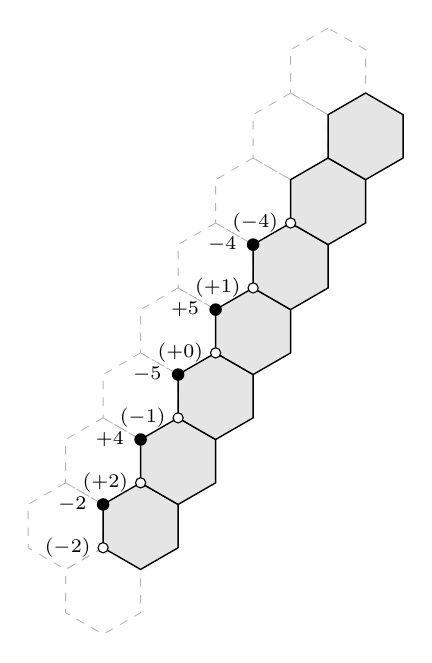
\begin{tikzpicture}[scale=0.55]
  \draw[fill=none,draw=black!30,line width=0.3pt,dashed] (-1.732,1.000) -- (-2.598,0.500) -- (-2.598,-0.500) -- (-1.732,-1.000) -- (-0.866,-0.500) -- (-0.866,0.500) -- cycle;
  \draw[fill=none,draw=black!30,line width=0.3pt,dashed] (-0.866,-0.500) -- (-1.732,-1.000) -- (-1.732,-2.000) -- (-0.866,-2.500) -- (-0.000,-2.000) -- (0.000,-1.000) -- cycle;
  \draw[fill=none,draw=black!30,line width=0.3pt,dashed] (-0.866,2.500) -- (-1.732,2.000) -- (-1.732,1.000) -- (-0.866,0.500) -- (-0.000,1.000) -- (0.000,2.000) -- cycle;
  \draw[fill=none,draw=black!30,line width=0.3pt,dashed] (0.000,4.000) -- (-0.866,3.500) -- (-0.866,2.500) -- (-0.000,2.000) -- (0.866,2.500) -- (0.866,3.500) -- cycle;
  \draw[fill=none,draw=black!30,line width=0.3pt,dashed] (0.866,5.500) -- (-0.000,5.000) -- (0.000,4.000) -- (0.866,3.500) -- (1.732,4.000) -- (1.732,5.000) -- cycle;
  \draw[fill=none,draw=black!30,line width=0.3pt,dashed] (1.732,7.000) -- (0.866,6.500) -- (0.866,5.500) -- (1.732,5.000) -- (2.598,5.500) -- (2.598,6.500) -- cycle;
  \draw[fill=none,draw=black!30,line width=0.3pt,dashed] (2.598,8.500) -- (1.732,8.000) -- (1.732,7.000) -- (2.598,6.500) -- (3.464,7.000) -- (3.464,8.000) -- cycle;
  \draw[fill=none,draw=black!30,line width=0.3pt,dashed] (3.464,10.000) -- (2.598,9.500) -- (2.598,8.500) -- (3.464,8.000) -- (4.330,8.500) -- (4.330,9.500) -- cycle;
  \draw[fill=none,draw=black!30,line width=0.3pt,dashed] (4.330,11.500) -- (3.464,11.000) -- (3.464,10.000) -- (4.330,9.500) -- (5.196,10.000) -- (5.196,11.000) -- cycle;
  \draw[fill=black!10,draw=black,line width=0.5pt] (0.000,1.000) -- (-0.866,0.500) -- (-0.866,-0.500) -- (-0.000,-1.000) -- (0.866,-0.500) -- (0.866,0.500) -- cycle;
  \draw[fill=black!10,draw=black,line width=0.5pt] (0.866,2.500) -- (-0.000,2.000) -- (0.000,1.000) -- (0.866,0.500) -- (1.732,1.000) -- (1.732,2.000) -- cycle;
  \draw[fill=black!10,draw=black,line width=0.5pt] (1.732,4.000) -- (0.866,3.500) -- (0.866,2.500) -- (1.732,2.000) -- (2.598,2.500) -- (2.598,3.500) -- cycle;
  \draw[fill=black!10,draw=black,line width=0.5pt] (2.598,5.500) -- (1.732,5.000) -- (1.732,4.000) -- (2.598,3.500) -- (3.464,4.000) -- (3.464,5.000) -- cycle;
  \draw[fill=black!10,draw=black,line width=0.5pt] (3.464,7.000) -- (2.598,6.500) -- (2.598,5.500) -- (3.464,5.000) -- (4.330,5.500) -- (4.330,6.500) -- cycle;
  \draw[fill=black!10,draw=black,line width=0.5pt] (4.330,8.500) -- (3.464,8.000) -- (3.464,7.000) -- (4.330,6.500) -- (5.196,7.000) -- (5.196,8.000) -- cycle;
  \draw[fill=black!10,draw=black,line width=0.5pt] (5.196,10.000) -- (4.330,9.500) -- (4.330,8.500) -- (5.196,8.000) -- (6.062,8.500) -- (6.062,9.500) -- cycle;
  \node[circle,fill=black,inner sep=1.6pt,label={left:$\scriptstyle -2$}] at (-0.866,0.500) {};
  \node[circle,fill=black,inner sep=1.6pt,label={left:$\scriptstyle +4$}] at (0.000,2.000) {};
  \node[circle,fill=black,inner sep=1.6pt,label={left:$\scriptstyle -5$}] at (0.866,3.500) {};
  \node[circle,fill=black,inner sep=1.6pt,label={left:$\scriptstyle +5$}] at (1.732,5.000) {};
  \node[circle,fill=black,inner sep=1.6pt,label={left:$\scriptstyle -4$}] at (2.598,6.500) {};
  \node[circle,draw=black,fill=white,inner sep=1.3pt,label={[label distance=-1pt]left:$\scriptstyle (-2)$}] at (-0.866,-0.500) {};
  \node[circle,draw=black,fill=white,inner sep=1.3pt,label={[label distance=-1pt]left:$\scriptstyle (+2)$}] at (0.000,1.000) {};
  \node[circle,draw=black,fill=white,inner sep=1.3pt,label={[label distance=-1pt]left:$\scriptstyle (-1)$}] at (0.866,2.500) {};
  \node[circle,draw=black,fill=white,inner sep=1.3pt,label={[label distance=-1pt]left:$\scriptstyle (+0)$}] at (1.732,4.000) {};
  \node[circle,draw=black,fill=white,inner sep=1.3pt,label={[label distance=-1pt]left:$\scriptstyle (+1)$}] at (2.598,5.500) {};
  \node[circle,draw=black,fill=white,inner sep=1.3pt,label={[label distance=-1pt]left:$\scriptstyle (-4)$}] at (3.464,7.000) {};
\end{tikzpicture}
\caption{The worked example of Example~\ref{ex:chain}.  The heptacene core
is rooted at its bottom cell; the dashed cells lie outside $\Lambda^{+}$.  Filled
vertices carry the entries of the witness $\Zy$, and the hollow vertices are
the white vertices $w$ at which $\lVert A\Zy\rVert^2$ is evaluated, labelled
by the sums $s_w$ in parentheses.}
\label{fig:chain}
\end{figure}

Most patterns are less simple than Example~\ref{ex:chain}.  The witnesses of
the certificate have between $7$ and $15$ nonzero entries, with $13$ the
commonest number, and most patterns need some cells of the collar to be
forced present or forced absent before the integer inequality
\eqref{eq:certificate} holds; this is exactly why a cover is needed.  The
pattern of Example~\ref{ex:chain} is not one of the $22{,}009$, and we give
it because it is small enough to be checked by hand: the certificate is not
claimed to be minimal, and shorter witnesses exist for many of its cores.

\subsection{The cover}\label{sec:cover}

What follows is the standard first-failure branching of a backtracking search
over the occupancy patterns, recorded as a static object so that it can be
checked rather than re-run.

The occupancy patterns are the vertices of a Boolean cube of dimension $85$,
with one coordinate for each cell of the window.
A \textsl{subcube} is a pair $\cQ=(U^{+},U^{-})$ of disjoint subsets of $W_7$,
and an occupancy pattern $\Omega$ \textsl{lies in} $\cQ$ if $U^{+}\sbs \Omega$ and
$U^{-}\cap \Omega=\varnothing$.  The cells of $U^{+}$ are the cells that $\cQ$
declares present and those of $U^{-}$ are the cells it declares absent; the
remaining cells of $W_7$ are the cells undecided by $\cQ$.
The \textsl{literals} of a decorated pattern
$P=(C;P^{+},P^{-};\Zy)$ are the statements ``$c$ is present'' for $c\in P^{+}$
and ``$c$ is absent'' for $c\in P^{-}$; an occupancy pattern matches $P$
exactly when it satisfies all the literals of $P$.  A literal of $P$ is
\textsl{decided} by a subcube $\cQ$ if it is satisfied or violated by every
occupancy pattern in $\cQ$, and \textsl{undecided} otherwise; $P$ is
\textsl{consistent} with $\cQ$ if none of its literals is violated by every
occupancy pattern in $\cQ$.

Suppose $P$ is consistent with $\cQ$ and let $\ell_1,\ldots,\ell_m$ be the
literals of $P$ undecided by $\cQ$, listed in a fixed order.  Then the
occupancy patterns in $\cQ$ are partitioned into $m+1$ classes: those
satisfying all of $\ell_1,\ldots,\ell_m$, which match $P$; and, for each
$i=1,\ldots,m$, those satisfying $\ell_1,\ldots,\ell_{i-1}$ and violating
$\ell_i$.  Each of the latter classes is again the set of occupancy patterns
in a subcube, which we denote $\cQ_i$; it is obtained from $\cQ$ by deciding the
cells of $\ell_1,\ldots,\ell_i$, with $\ell_i$ decided the wrong way.  We
will call $\cQ_1,\ldots,\cQ_m$ the \textsl{first-failure children} of
$(P,\cQ)$.

The \textsl{cover} is a directed acyclic graph.  Each node stores a robust
obstruction pattern $P$ and a subcube $\cQ$ consistent with $P$, and its
out-neighbours are nodes whose subcubes are exactly the first-failure children
of $(P,\cQ)$, one for each child.  A node is a \textsl{leaf} if $P$ has no
literal undecided by $\cQ$.  For each rooted core $C_0$ there is a
\textsl{root} node whose subcube is $(C_0,\varnothing)$: the seven cells of
$C_0$ are present and the remaining $78$ cells of $W_7$ are undecided.
Nodes may have several in-neighbours; subproblems that arise more than once
are shared.  The certificate consists of
\begin{equation}\label{eq:certificate-counts}
 3{,}652\text{ rooted cores},\qquad
 22{,}009\text{ robust obstruction patterns},\qquad
 345{,}554\text{ cover nodes}.
\end{equation}

\begin{example}\label{ex:node}
We give one node of the cover, taken from the certificate, together with its
children; it is drawn in Figure~\ref{fig:node}.  Let
\[
 C_0=\{(0,0),\,(0,1),\,(0,2),\,(1,0),\,(1,1),\,(1,2),\,(2,0)\}
\]
be a rooted core, and consider its root node, whose subcube is
$\cQ=(C_0,\varnothing)$: the seven cells of $C_0$ are present and the other
$78$ cells of $W_7$ are undecided.  The pattern $P$ stored at this node has
core $C_0$, with $P^{+}=C_0$ and $P^{-}=\{(1,-1),(2,-1)\}$, two cells of the
collar of $C_0$.  Its witness has thirteen nonzero entries, and
\[
\begin{aligned}
 &N=\Zy\tp\Zy=104,\qquad M=-\widehat q_P(\Zy)=186,\\
 &2M-N=268>0,\qquad 5N^{2}=54{,}080<71{,}824=(2M-N)^{2},
\end{aligned}
\]
so $P$ is a robust obstruction pattern.

The pattern $P$ has nine literals.  The subcube decides the seven that assert
that the cells of $C_0$ are present, and leaves two undecided: $\ell_1$, that
$(1,-1)$ is absent, and $\ell_2$, that $(2,-1)$ is absent.  The node
therefore has two first-failure children.  The first is the subcube in which
$(1,-1)$ is present and nothing else has been decided beyond $C_0$, and the
second is the subcube in which $(1,-1)$ is absent and $(2,-1)$ is present.  Both
children are leaves.  The pattern stored at the first has core
\[
 \{(0,0),\,(0,1),\,(0,2),\,(1,-1),\,(1,0),\,(1,1),\,(1,2)\} ,
\]
which is $C_0$ with $(2,0)$ traded for $(1,-1)$, and the pattern stored at
the second has core
\[
 \{(0,0),\,(0,1),\,(0,2),\,(1,0),\,(1,1),\,(1,2),\,(2,-1)\} ,
\]
which is $C_0$ with $(2,0)$ traded for $(2,-1)$.  Neither of these two
patterns has any literal beyond the seven cells of its own core, so each of
them is a leaf under every subcube containing its core, and three patterns
between them handle every occupancy pattern containing $C_0$.  The two
literals $\ell_1$ and $\ell_2$ are what the integer inequality
\eqref{eq:certificate} needs
rather than what the geometry needs: $C_0$ is in fact an obstruction in the
polyhex $C_0\cup\{(1,-1)\}$ as well, but the relaxation $\widehat q_P$ does
not certify it there.  In the certificate this is core $280$ and node $599$,
storing pattern $513$, with leaves $416$ and $598$ storing patterns $342$ and
$512$.
\end{example}

\begin{figure}[ht]
\centering
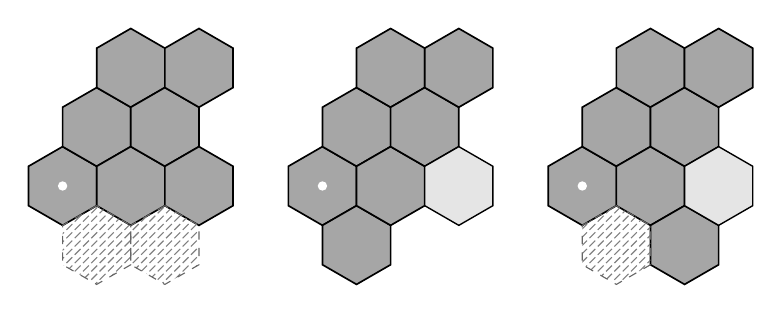
\begin{tikzpicture}[scale=0.50]
\begin{scope}[shift={(0.00,0)}]
  \draw[fill=black!35,draw=black,line width=0.6pt] (0.000,1.000) -- (-0.866,0.500) -- (-0.866,-0.500) -- (0.000,-1.000) -- (0.866,-0.500) -- (0.866,0.500) -- cycle;
  \draw[fill=black!35,draw=black,line width=0.6pt] (0.866,2.500) -- (0.000,2.000) -- (0.000,1.000) -- (0.866,0.500) -- (1.732,1.000) -- (1.732,2.000) -- cycle;
  \draw[fill=black!35,draw=black,line width=0.6pt] (1.732,4.000) -- (0.866,3.500) -- (0.866,2.500) -- (1.732,2.000) -- (2.598,2.500) -- (2.598,3.500) -- cycle;
  \draw[fill=black!35,draw=black,line width=0.6pt] (1.732,1.000) -- (0.866,0.500) -- (0.866,-0.500) -- (1.732,-1.000) -- (2.598,-0.500) -- (2.598,0.500) -- cycle;
  \draw[fill=black!35,draw=black,line width=0.6pt] (2.598,2.500) -- (1.732,2.000) -- (1.732,1.000) -- (2.598,0.500) -- (3.464,1.000) -- (3.464,2.000) -- cycle;
  \draw[fill=black!35,draw=black,line width=0.6pt] (3.464,4.000) -- (2.598,3.500) -- (2.598,2.500) -- (3.464,2.000) -- (4.330,2.500) -- (4.330,3.500) -- cycle;
  \draw[fill=black!35,draw=black,line width=0.6pt] (3.464,1.000) -- (2.598,0.500) -- (2.598,-0.500) -- (3.464,-1.000) -- (4.330,-0.500) -- (4.330,0.500) -- cycle;
  \draw[pattern=north east lines,pattern color=black!50,draw=black!60,line width=0.4pt,dashed] (0.866,-0.500) -- (0.000,-1.000) -- (0.000,-2.000) -- (0.866,-2.500) -- (1.732,-2.000) -- (1.732,-1.000) -- cycle;
  \draw[pattern=north east lines,pattern color=black!50,draw=black!60,line width=0.4pt,dashed] (2.598,-0.500) -- (1.732,-1.000) -- (1.732,-2.000) -- (2.598,-2.500) -- (3.464,-2.000) -- (3.464,-1.000) -- cycle;
  \node[circle,fill=white,inner sep=1.2pt] at (0.000,0.000) {};
\end{scope}
\begin{scope}[shift={(6.60,0)}]
  \draw[fill=black!35,draw=black,line width=0.6pt] (0.000,1.000) -- (-0.866,0.500) -- (-0.866,-0.500) -- (0.000,-1.000) -- (0.866,-0.500) -- (0.866,0.500) -- cycle;
  \draw[fill=black!35,draw=black,line width=0.6pt] (0.866,2.500) -- (0.000,2.000) -- (0.000,1.000) -- (0.866,0.500) -- (1.732,1.000) -- (1.732,2.000) -- cycle;
  \draw[fill=black!35,draw=black,line width=0.6pt] (1.732,4.000) -- (0.866,3.500) -- (0.866,2.500) -- (1.732,2.000) -- (2.598,2.500) -- (2.598,3.500) -- cycle;
  \draw[fill=black!35,draw=black,line width=0.6pt] (0.866,-0.500) -- (0.000,-1.000) -- (0.000,-2.000) -- (0.866,-2.500) -- (1.732,-2.000) -- (1.732,-1.000) -- cycle;
  \draw[fill=black!35,draw=black,line width=0.6pt] (1.732,1.000) -- (0.866,0.500) -- (0.866,-0.500) -- (1.732,-1.000) -- (2.598,-0.500) -- (2.598,0.500) -- cycle;
  \draw[fill=black!35,draw=black,line width=0.6pt] (2.598,2.500) -- (1.732,2.000) -- (1.732,1.000) -- (2.598,0.500) -- (3.464,1.000) -- (3.464,2.000) -- cycle;
  \draw[fill=black!35,draw=black,line width=0.6pt] (3.464,4.000) -- (2.598,3.500) -- (2.598,2.500) -- (3.464,2.000) -- (4.330,2.500) -- (4.330,3.500) -- cycle;
  \draw[fill=black!10,draw=black,line width=0.5pt] (3.464,1.000) -- (2.598,0.500) -- (2.598,-0.500) -- (3.464,-1.000) -- (4.330,-0.500) -- (4.330,0.500) -- cycle;
  \node[circle,fill=white,inner sep=1.2pt] at (0.000,0.000) {};
\end{scope}
\begin{scope}[shift={(13.20,0)}]
  \draw[fill=black!35,draw=black,line width=0.6pt] (0.000,1.000) -- (-0.866,0.500) -- (-0.866,-0.500) -- (0.000,-1.000) -- (0.866,-0.500) -- (0.866,0.500) -- cycle;
  \draw[fill=black!35,draw=black,line width=0.6pt] (0.866,2.500) -- (0.000,2.000) -- (0.000,1.000) -- (0.866,0.500) -- (1.732,1.000) -- (1.732,2.000) -- cycle;
  \draw[fill=black!35,draw=black,line width=0.6pt] (1.732,4.000) -- (0.866,3.500) -- (0.866,2.500) -- (1.732,2.000) -- (2.598,2.500) -- (2.598,3.500) -- cycle;
  \draw[fill=black!35,draw=black,line width=0.6pt] (1.732,1.000) -- (0.866,0.500) -- (0.866,-0.500) -- (1.732,-1.000) -- (2.598,-0.500) -- (2.598,0.500) -- cycle;
  \draw[fill=black!35,draw=black,line width=0.6pt] (2.598,2.500) -- (1.732,2.000) -- (1.732,1.000) -- (2.598,0.500) -- (3.464,1.000) -- (3.464,2.000) -- cycle;
  \draw[fill=black!35,draw=black,line width=0.6pt] (3.464,4.000) -- (2.598,3.500) -- (2.598,2.500) -- (3.464,2.000) -- (4.330,2.500) -- (4.330,3.500) -- cycle;
  \draw[fill=black!35,draw=black,line width=0.6pt] (2.598,-0.500) -- (1.732,-1.000) -- (1.732,-2.000) -- (2.598,-2.500) -- (3.464,-2.000) -- (3.464,-1.000) -- cycle;
  \draw[fill=black!10,draw=black,line width=0.5pt] (3.464,1.000) -- (2.598,0.500) -- (2.598,-0.500) -- (3.464,-1.000) -- (4.330,-0.500) -- (4.330,0.500) -- cycle;
  \draw[pattern=north east lines,pattern color=black!50,draw=black!60,line width=0.4pt,dashed] (0.866,-0.500) -- (0.000,-1.000) -- (0.000,-2.000) -- (0.866,-2.500) -- (1.732,-2.000) -- (1.732,-1.000) -- cycle;
  \node[circle,fill=white,inner sep=1.2pt] at (0.000,0.000) {};
\end{scope}
\end{tikzpicture}
\caption{The node of Example~\ref{ex:node} and its two first-failure
children, with the origin marked by a white dot.  In each drawing the core of
the stored pattern is dark, a cell declared present by the subcube but not in
that core is light, and a hatched cell is one declared absent; the cells of
$W_7$ that are not drawn are undecided.  Left: the root node for $C_0$, whose
pattern forces the two collar cells $(1,-1)$ and $(2,-1)$ absent.  Centre:
the child in which $(1,-1)$ is present.  Right: the child in which $(1,-1)$
is absent and $(2,-1)$ is present.  In each child the core that carries the
witness is a different seven-cell set.}
\label{fig:node}
\end{figure}

\begin{lemma}\label{lem:cover}
Let $C_0$ be a rooted core and let $\Omega$ be an occupancy pattern containing
$C_0$.  Then $\Omega$ matches the pattern stored at some node of the cover.
\end{lemma}

\begin{proof}
We show by induction on the number of undecided cells of the subcube that every
occupancy pattern lying in the subcube of a node matches the pattern stored at
that node or at some node reachable from it.  At a leaf every literal of $P$
is decided by $\cQ$; since $P$ is consistent with $\cQ$, no literal of $P$ is
violated by every occupancy pattern in $\cQ$, and a decided literal is either
satisfied by all of them or violated by all of them, so every literal of $P$
is satisfied by every occupancy pattern in $\cQ$.  Thus at a leaf every
occupancy pattern in the subcube matches the stored pattern.  At a node
$(P,\cQ)$ that is
not a leaf, an occupancy pattern in $\cQ$ either matches $P$, or has a first
undecided literal of $P$ that it violates and so lies in a first-failure
child, which is the subcube of an out-neighbour and has strictly fewer
undecided cells.  Since $\Omega$ lies in the subcube $(C_0,\varnothing)$ of the root
node for $C_0$, the statement follows.
\end{proof}

\begin{proof}[Proof of Theorem~\ref{thm:seven}]
Let $H$ be a polyhex with at least seven cells, translated so that its
lexicographically first cell is the origin.  As
observed in Section~\ref{sec:rooting}, $H$ contains a rooted core $C_0$, and
so the occupancy pattern $\Omega=H\cap W_7$ contains $C_0$.  By
Lemma~\ref{lem:cover}, $\Omega$ matches some robust obstruction pattern
$P=(C;P^{+},P^{-};\Zy)$ of the cover.  Then $H$ matches $P$, and
$C\sbs P^{+}\sbs H$ is a connected set of exactly seven cells.  The core of a
decorated pattern is a rooted core, so $(0,0)\in C$.  By
Lemma~\ref{lem:pattern-works}, $\Zy\tp M_C(H)\Zy<0$, so $C$ is an
obstruction in $H$.
\end{proof}

\begin{remark}\label{rem:core-changes}
The core $C$ supplied by the cover need not be the core $C_0$ we started
from, and this freedom is essential rather than cosmetic.  In the
configuration of Figure~\ref{fig:window}, the coronene core is not an
obstruction, and the cover certifies the configuration through a different
seven-cell set inside the same $85$-cell window.
\end{remark}

\begin{remark}\label{rem:compress}
The certificate is sufficient and has been verified exactly, but it is not
claimed to be minimal, irredundant or in any sense canonical.  Both the
number of patterns and the sizes of their witnesses can be reduced, at the
cost of a larger cover.  We report the certificate as it stands because it
is the one that has been verified.
\end{remark}

\section{Polyhexes with at most six hexagons}\label{sec:small}

Generate all polyhexes with at most six cells, up to translations and the
dihedral symmetries of the tiling, by adjoining one adjacent cell at a time
and canonicalizing.  The counts are
\begin{equation}\label{eq:small-counts}
 1,\ 1,\ 3,\ 7,\ 22,\ 82
\end{equation}
for $h=1,\ldots,6$, a total of $116$ polyhexes; the ring of six cells around
a hole is amongst them.  Exactly three of the $116$ lie in the golden gap
class, and the two cases call for opposite kinds of evidence: for the others
we exhibit a witness, and for these three we must certify that none exists.

\subsection{The hundred and thirteen that are not in the class}

Let $H$ be one of the $113$ polyhexes that are not in the golden gap class,
with graph $X$ and adjacency matrix $A$, and let $\Zy$ be a nonzero integer
vector supported on one colour class of $X$.  Here $H$ is completely known,
so nothing plays the role that $\widehat q_P$ played in
Section~\ref{sec:patterns}: the quantity $\Zy\tp(A^{2}-2I)\Zy$ is computed
exactly.  Put
\[
 N=\Zy\tp\Zy,\qquad M=-\,\Zy\tp\bigl(A^{2}-2I\bigr)\Zy ,
\]
both integers, with $N>0$.  Since $\thetaG^{2}=2-\vphi$, we have
$\Zy\tp(A^{2}-\thetaG^{2}I)\Zy=\vphi N-M$, so $\Zy$ witnesses that
$A^{2}-\thetaG^{2}I$ is not positive semidefinite precisely when $\vphi N<M$,
which by \eqref{eq:certificate} is the pair of integer inequalities
\begin{equation}\label{eq:small-certificate}
 2M-N>0\qquad\text{and}\qquad 5N^{2}<(2M-N)^{2}.
\end{equation}

Such a $\Zy$ exists for each of the $113$.  Indeed $A^{2}$ is block diagonal
with respect to the two colour classes, so one of the two blocks fails to be
positive semidefinite, and a witness supported on a single colour class is
obtained from an eigenvector of that block for a negative eigenvalue by
rounding and scaling.  We record one for each of the $113$.  They are small:
each has at most $11$ nonzero entries, no entry exceeds $4$ in absolute
value, and $69$ of the $113$ have every entry equal to $\pm1$.  The largest
integer occurring in \eqref{eq:small-certificate} anywhere among them is
$12{,}544$.

\subsection{The three that are}

For benzene, naphthalene and triphenylene we give the characteristic
polynomial and its factorization over $\ints$.  Writing $\chi$ for the
characteristic polynomial,
\[
\begin{aligned}
 \chi_{\text{benzene}}&=(x-2)(x+2)(x-1)^{2}(x+1)^{2},\\
 \chi_{\text{naphthalene}}&=(x-1)(x+1)(x^{2}-x-3)(x^{2}+x-3)(x^{2}-x-1)(x^{2}+x-1),\\
 \chi_{\text{triphenylene}}&=(x^{3}-3x^{2}+3)(x^{3}+3x^{2}-3)(x^{6}-6x^{4}+9x^{2}-3)^{2}.
\end{aligned}
\]
The smallest positive root of $\chi_{\text{benzene}}$ is $1$.  Now
$\thetaG$ is the positive root of $x^{2}+x-1$, so $\thetaG$ is a root of
$\chi_{\text{naphthalene}}$, and it is the smallest positive one; naphthalene
is therefore in the golden gap class and attains $\thetaG$.  The smallest
positive root of $\chi_{\text{triphenylene}}$ is the root
$0.684040\ldots>\thetaG$ of the sextic factor $x^{6}-6x^{4}+9x^{2}-3$.  Each
of these statements is a finite check on integer polynomials: it suffices to
evaluate each factor at $\thetaG$ in $\ints[\vphi]$, where $\thetaG=\vphi-1$,
and to count roots in $(0,\thetaG]$.

\begin{proposition}\label{prop:small}
Exactly three of the $116$ polyhexes with at most six cells lie in the
golden gap class: benzene, naphthalene, and the four-cell benzenoid with
cells $(0,1),(1,1),(1,2),(2,0)$, which is triphenylene.
\end{proposition}

\begin{proof}
For each of the other $113$, the recorded witness satisfies
\eqref{eq:small-certificate}, so by Lemma~\ref{lem:reduction} its graph has
an eigenvalue in $(-\thetaG,\thetaG)$.  For the three named, the
factorizations above show that no eigenvalue lies in that interval.
\end{proof}

Every comparison in this section is therefore between integers, apart from
the three characteristic polynomials, whose roots are classical.  As an
independent cross-check we also decide positive semidefiniteness of the two
matrices $RR\tp-\thetaG^2I$ and $R\tp R-\thetaG^2I$ of
Lemma~\ref{lem:reduction} directly, for all $116$ polyhexes, by symmetric
Gaussian elimination pivoting on positive diagonal entries and carried out
exactly over $\rats(\sqrt5)$: each entry is stored as $(a+b\vphi)/c$ with
arbitrary precision integers $a,b,c$, and the sign of each entry is decided
exactly.  At each step we inspect the diagonal of the block that remains.  A
negative diagonal entry certifies failure.  A zero diagonal entry of a
positive semidefinite matrix forces its row and its column to vanish, so if
every remaining diagonal entry is zero we return positive semidefinite
exactly when the whole remaining block is zero.  Otherwise we pivot on a
positive diagonal entry, which leaves a smaller symmetric block, and repeat.
This decides positive semidefiniteness and not merely positive definiteness,
and the distinction is exactly what is needed here: naphthalene is the
equality case, so its blocks are singular and the elimination stalls on them.
The two computations agree.

\begin{proof}[Proof of Theorem~\ref{thm:gap}]
Let $H$ be a polyhex.  If $H$ has at least seven cells, then by
Theorem~\ref{thm:seven} it contains an obstruction, and by
Lemmas~\ref{lem:principal} and \ref{lem:reduction} its graph has an
eigenvalue in $(-\thetaG,\thetaG)$.  If $H$ has at most six cells, then by
Proposition~\ref{prop:small} and Lemma~\ref{lem:reduction} it lies in the
golden gap class if and only if it is benzene, naphthalene or triphenylene.
\end{proof}

\section{Verification}\label{sec:verification}

We now describe what was computed, how it was checked, and what the
computation does not establish.  The certificate, the verifiers and the
transcripts of their runs accompany this paper.%
\footnote{Available from the author; the files will also be placed in a
public repository with a DOI, which will be inserted here.}

\subsection*{The certificate and its verifier}

The certificate is a text file listing the $85$ cells of $W_7$, the
$3{,}652$ rooted cores, and the $22{,}009$ robust obstruction patterns,
together with a binary file encoding the $345{,}554$ nodes of the cover.
The two files and their SHA-256 digests are
\begin{center}\footnotesize
\begin{tabular}{@{}l@{}}
\texttt{seven\_hexagon\_obstructions.txt}\\
\texttt{37936464fe433b52987dad9f5c2f186de52fc6ef0850c976d778d0c9a755ab78}\\[3pt]
\texttt{seven\_hexagon\_cover.bin}\\
\texttt{51183fa42b2592ebd276e793a7d9ba9b7bc7a0f8633db4a5fc536e4b177fbb6b}
\end{tabular}
\end{center}
so that the transcripts quoted below are tied to exact bytes.

The two formats are specified in Appendix~\ref{app:spec}, in enough detail
to be read without reference to our code.

The certificate is checked by
\texttt{seven\_\allowbreak hexagon\_\allowbreak exact\_\allowbreak verify.cpp},
a C\texttt{++} program of about $350$ lines which does not trust the search
that produced it.  The program
\begin{enumerate}
\item[(i)] reconstructs $W_6$ and $W_7$ and verifies the counts
 \eqref{eq:W-counts}, and enumerates the rooted cores independently and
 compares them, in order, with those listed;
\item[(ii)] for each pattern, re-derives the collar of its core, checks
 that $P^{+}$ and $P^{-}$ are disjoint subsets of $W_7$ lying in the core or
 its collar with $C\sbs P^{+}$, checks that the witness is a nonzero integer
 vector supported on vertices of one colour, recomputes
 $\widehat q_P(\Zy)$ from \eqref{eq:qhat}, and checks the strict integer
 inequality \eqref{eq:certificate} in arbitrary precision integer
 arithmetic;
\item[(iii)] checks that every node of the cover stores a listed pattern
 consistent with its subcube, that its out-neighbours carry exactly the
 first-failure children of the node, and that every rooted core has a root
 node with subcube $(C_0,\varnothing)$; and
\item[(iv)] generates the $116$ polyhexes with at most six cells, verifies
 the counts \eqref{eq:small-counts}, and decides positive semidefiniteness
 of the two colour blocks of each exactly over $\rats(\sqrt5)$, by the
 symmetric Gaussian elimination, pivoting on positive diagonal entries,
 described in Section~\ref{sec:small}, reporting the survivors.  This is the
 cross-check of Section~\ref{sec:small}; the witnesses of
 \eqref{eq:small-certificate} are checked separately, as described below.
\end{enumerate}
The run takes under two seconds and reports the three survivors of
Proposition~\ref{prop:small}.  Arbitrary precision integers are supplied by
the Boost multiprecision library or, equivalently, by GMP; the program has
been compiled and run with both, with identical output.  Machine integers
would in fact suffice.  If the support of $\Zy$ has size $s$ and its entries
are at most $b$ in absolute value, then at most $3s$ white vertices of the
tiling meet the support and each of them contributes at most $(3b)^{2}$ to
the first sum in \eqref{eq:qhat}, since every vertex of the tiling has degree
three; thus $M=\abs{\widehat q_P(\Zy)}\le27sb^{2}$ and $N=\Zy\tp\Zy\le sb^{2}$,
so $0<2M-N\le55sb^{2}$ and both sides of the second inequality in
\eqref{eq:certificate} are at most $(55sb^{2})^{2}$.  In the certificate
every witness has $s\le15$ and $b\le179$, the largest value of $N$ is
$89{,}954$ and the largest value of $2M-N$ is $201{,}144$, so the largest
integer actually compared is $4.05\cdot10^{10}$ and no overflow of a $64$-bit
integer is possible.  We keep the arbitrary precision arithmetic as belt and
braces.  The transcript of the run against GMP is the file
\texttt{seven\_hexagon\_verification\_gmp\_rerun.log}.

\subsection*{Independent re-verification}

A second verifier,
\texttt{seven\_\allowbreak hexagon\_\allowbreak reverify.py}, written in Python
from the specification of
Sections~\ref{sec:seven} and \ref{sec:small} rather than from the
C\texttt{++} source, repeats checks (i) to (iii) and then performs tests of a
different kind.  It draws a rooted core and a random occupancy pattern of
$W_7$ containing it, routes the occupancy pattern through the cover to the
node whose stored pattern it matches, and then computes the block $M_C$ of
that pattern's core directly and exactly over $\rats(\sqrt5)$, without
reference to the witness, and confirms that it is not positive semidefinite.
Two thousand such end-to-end tests were run on the $22{,}009$-pattern
certificate with no disagreement; the transcript is the file
\texttt{seven\_hexagon\_reverify\_shipped\_2000.log}.
Separately, for each of the $333+1448+6572=8{,}353$ polyhexes with seven,
eight or nine cells, a connected seven-cell obstruction containing the
lexicographically first cell was found by direct exact computation, by the
program \texttt{seven\_\allowbreak hexagon\_\allowbreak optimality.py},
which also carries out the exact checks behind
Proposition~\ref{prop:nosix}; the transcript is the file
\texttt{seven\_hexagon\_statement\_scan\_h9.log}.  This is
the conclusion of Theorem~\ref{thm:seven} in the rooted form in which we have
stated it.

The integer witnesses of Section~\ref{sec:small} are shipped as the file
\texttt{small\_polyhex\_witnesses.txt}, which also records the
characteristic polynomials and their factorizations for the three members of
the golden gap class.  A third verifier,
\texttt{small\_polyhex\_verify.py}, regenerates the $116$ polyhexes
independently, checks the counts \eqref{eq:small-counts}, and verifies each
of the $113$ witnesses against \eqref{eq:small-certificate} in integer
arithmetic, recomputing $N$ and $M$ from the adjacency matrix; it then checks
the three factorizations and locates the smallest positive root of each
exactly.  It uses no library beyond the Python standard library.  The
transcript is the file \texttt{small\_polyhex\_verify.log}.

The exact checks of Proposition~\ref{prop:nosix} were carried out in the same
exact arithmetic, and the numerical values quoted in this paper were computed
in double precision as a cross-check.

\subsection*{What the computation does not establish}

The certificate, and not the search that produced it, is the object of
record.  Nothing in this paper depends on how the cores, the patterns or the
cover were found: the verifier of Section~\ref{sec:verification} rebuilds
$W_6$ and $W_7$, re-enumerates the rooted cores, recomputes every
$\widehat q_P(\Zy)$ and every integer inequality, and re-derives the
first-failure partition at every node, so a search that was mistaken, or
adversarial, could not produce data that passes.  We therefore make no claim
about the search, and none is needed.

The computation establishes that the data satisfies the specification of
Sections~\ref{sec:rooting} to \ref{sec:cover}.  It does not, and cannot,
check the specification itself, which consists of five facts: that a polyhex
rooted at its lexicographically first cell lies in $\Lambda^{+}$, which is
\eqref{eq:halfplane} and is immediate from the definition of the
lexicographic order; that the collar of a rooted core lies in $W_7$, which is
Lemma~\ref{lem:local}; that $\widehat q_P$ bounds the quadratic form, which
is Lemma~\ref{lem:qhat}; that the integer inequality
\eqref{eq:certificate} gives $\Zy\tp M_C(H)\Zy<0$ for every rooted polyhex
$H$ matching the pattern, which is Lemma~\ref{lem:pattern-works}; and that
the first-failure children partition a subcube, which is
Lemma~\ref{lem:cover}.  These proofs are short and are given in full above.
The second verifier is independent code but was written from the same
specification, so on its own it detects errors in the data rather than in
the specification.  The end-to-end tests and the scan of polyhexes with at
most nine cells are the checks that bypass the specification, since they
compare the conclusion of Theorem~\ref{thm:seven} against exact spectra
computed directly.


\section*{Declaration on the use of AI tools}

The strategy of the proof is the author's: to prove the stronger statement,
Theorem~\ref{thm:gap}, rather than Corollary~\ref{cor:pisanski}, by
exhibiting a local block of $A^2-\thetaG^2I$ that is not positive
semidefinite, following the approach of Guo and Royle \cite{GuoRoy2024}.
The computations showing that six hexagons do not suffice
(Section~\ref{sec:optimality}) were carried out by the author with the
assistance of Claude (Anthropic).

The argument for seven hexagons in Section~\ref{sec:seven} is not the
author's.  The author's plan for this step rested on a much larger case
analysis.  A draft of the paper containing that plan and a proof sketch of a much more computationally-dependent proof with more case analysis was given to ChatGPT~5.6
Pro (OpenAI), which completed it with a different argument, including Lemmas~\ref{lem:local}, \ref{lem:qhat}, \ref{lem:pattern-works}
and~\ref{lem:cover}, none of which the author had drafted.  This argument
is shorter than the author's original one and a forthcoming edition will reconcile the two approaches to give a more intuitive proof.
Claude was also used in editing the text of the manuscript.



\appendix

\section{Specification of the certificate}\label{app:spec}

This appendix says what the two files contain and how they are to be read,
what a verifier must recompute, and how a certificate may be searched for.
It is meant to be enough to rebuild all of it from nothing.  We stress at the
outset that the search needs no correctness argument of any kind: whatever
produces the files, the checks of Section~\ref{sec:verification} are applied
to them afterwards, and data that is wrong in any respect fails those checks.

\subsection{Conventions}

Cells carry axial coordinates as in Section~\ref{sec:polyhexes}.  We place the
cell $(q,r)$ with its centre at the point $(2q+r,3r)$ of the plane, so that
its six vertices are that centre translated by
\[
 (1,1),\quad(0,2),\quad(-1,1),\quad(-1,-1),\quad(0,-2),\quad(1,-1),
\]
listed in cyclic order, and the six edges of the cell join consecutive
vertices in that list.  Every vertex of the tiling then has integer
coordinates $(x,y)$ with $y\not\equiv0\pmod 3$, two cells are adjacent exactly
when they share two vertices, and the colour of a vertex is $y\bmod3$, which
takes the values $1$ and $2$ and is constant on each colour class.  Each edge
of the tiling lies on exactly two cells, which is the fact the verifier uses
to decide whether an edge is present.

\subsection{The atlas file}

The atlas is a stream of whitespace-separated tokens.  It opens with the
magic word \texttt{SEVEN\_\allowbreak HEXAGON\_\allowbreak OBSTRUCTIONS\_\allowbreak V1} and then has three
counted sections.  The first is the token \texttt{W7}, the number $85$, and
then $85$ records \texttt{W}~$j$~$q$~$r$ giving the cells of $W_7$; the index
$j$ runs from $0$ and fixes the numbering of $W_7$ used everywhere else.  The
second is the token \texttt{CORES}, the number $3{,}652$, and then that many
records \texttt{C}~$j$ followed by the seven coordinate pairs of the $j$th
rooted core.  The third is the token \texttt{PATTERNS}, the number $22{,}009$,
and then that many pattern records.  A pattern record is
\[
\begin{aligned}
 &\texttt{P}\quad j\quad c\quad
  k_{+}\ b_1\cdots b_{k_{+}}\quad
  k_{-}\ b'_1\cdots b'_{k_{-}}\\
 &\qquad k\ x_1\,y_1\,c_1\ \cdots\ x_k\,y_k\,c_k ,
\end{aligned}
\]
where $j$ is the pattern's index, $c$ the index of its core, the $b_i$ are the
$W_7$-indices of the cells of $P^{+}$, the $b'_i$ those of $P^{-}$, and the
triples give the witness: $\Zy(x_i,y_i)=c_i$, and $\Zy$ vanishes elsewhere.
Note that a coefficient $c_i$ is permitted to be zero, so the number $k$ of
recorded entries is an upper bound for the size of the support and need not
equal it.

\subsection{The cover file}

All integers in the cover are unsigned and little-endian.  The file begins
with the eight bytes \texttt{7HEXCVR1}, followed by three $32$-bit integers:
the number of nodes, the number of rooted cores and the number of patterns.
The node records follow, one for each node in order of its index.  A node
record is a $32$-bit integer giving the index of the pattern stored at the
node, a $32$-bit integer giving the number $m$ of arcs leaving it, and then
$m$ arc records of six bytes each.  An arc record is one byte giving the
index in $W_7$ of the cell of the corresponding literal, one byte giving the
value that the literal asserts, namely $1$ for present and $0$ for absent,
and a $32$-bit integer giving the index of the node carrying the
first-failure child in which that literal is violated.  The arcs of a node
are listed in the fixed order of the literals of its pattern that are
undecided by its subcube: those asserting presence first and then those
asserting absence, each group in increasing order of the index in $W_7$.  A
leaf has $m=0$.  The file ends with one $32$-bit integer for each of the
$3{,}652$ rooted cores, in the order in which the cores are listed in the
atlas, giving the index of the root node for that core.  There are no
trailing bytes, and a verifier should check that.

\subsection{Recomputing the bound}\label{app:qhat}

The one quantity a verifier must get exactly right is $\widehat q_P(\Zy)$,
and it is determined by the pattern alone.  It is defined by \eqref{eq:qhat};
we repeat here only what must be got right about the bookkeeping, and refer
to Section~\ref{sec:patterns} for the classification of edges itself.

Two conventions govern everything.  First, only the admissible collar
matters: a cell of the collar of $C$ that lies outside $\Lambda^{+}$ is
absent from every rooted polyhex and is to be treated as forced absent, never
as undetermined.  Equivalently, and this is the form to implement, build
$\collarp(C)$ rather than the full collar, record for each cell of it its
index in $W_7$, and let a cell carry no weight at all if it has no such
index.  Getting this wrong is the one error that silently inflates
$\widehat q_P(\Zy)$ and rejects a valid certificate.  Second, the cells of
$C$ itself are forced present, whether or not they are also listed in
$P^{+}$.

Concretely: build $\collarp(C)$, and record for each edge $e$ of the tiling
carried by $C$ or by $\collarp(C)$ a pair consisting of a flag saying whether
some cell of $C$ carries $e$, and the set of $W_7$-indices of the cells of
$\collarp(C)$ that carry $e$.  An edge with an empty record is discarded.
Now take each vertex $v$ in the support of $\Zy$ and each edge $vw$ at $v$,
classify it as forced, undetermined or discarded as in
Section~\ref{sec:patterns}, group the edges by $w$, and form $s_w$ and the
$t_{w,j}$.  Then $\widehat q_P(\Zy)$ is given by \eqref{eq:qhat}.  Since $w$
has three edges in the tiling, $k_w\le3$ and the maximum over $J$ may be
taken by inspecting at most eight subsets; alternatively, and this is worth
knowing for the search,
\begin{equation}\label{eq:qhat-twoway}
 \max_{J}\Bigl(s_w+\sum_{j\in J}t_{w,j}\Bigr)^{2}
 =\max\Bigl\{\bigl(s_w+\!\!\sum_{t_{w,j}>0}\!\!t_{w,j}\bigr)^{2},\
             \bigl(s_w+\!\!\sum_{t_{w,j}<0}\!\!t_{w,j}\bigr)^{2}\Bigr\},
\end{equation}
because $J\mapsto s_w+\sum_{j\in J}t_{w,j}$ is affine in the indicator of $J$
and so attains its largest and smallest values by taking all the positive
$t_{w,j}$ and all the negative ones respectively.

\subsection{Checking the cover}

A verifier walks the cover from each root.  At a node it recomputes, from the
node's subcube and the literals of the stored pattern, which literals are
undecided; it checks that none is violated by the whole subcube, so that the
pattern is consistent with it; and it checks that the arcs leaving the node
are exactly those literals, in the prescribed order, each leading to a node
whose subcube is the one obtained by deciding the literals up to and
including that one, with the last decided the wrong way.  A node reached
twice must carry the same subcube both times, and a verifier should check
that as well, since the cover is a directed acyclic graph with sharing and
not a tree.  Nothing else about the shape of the cover matters.

\subsection{Finding a certificate}\label{app:search}

We describe one method that works.  It is a heuristic and we make no claim
for it beyond that; its output is checked afterwards.

Fix a subcube, that is, a set of cells of $W_7$ declared present and a
disjoint set declared absent.  For a candidate core $C$ and a colour class,
\eqref{eq:qhat-twoway} turns the quantity we need to make negative into
\[
 \widehat q_P(\Zy)+\vphi\,\Zy\tp\Zy
 =\sum_{w}\max\bigl\{L^{+}_{w}(\Zy)^{2},\,L^{-}_{w}(\Zy)^{2}\bigr\}
   -\thetaG^{2}\,\Zy\tp\Zy ,
\]
using $2-\vphi=\thetaG^{2}$, where $L^{+}_{w}$ and $L^{-}_{w}$ are the two
linear forms obtained by adjoining to $s_w$ all the positive, respectively
all the negative, undetermined coefficients at $w$.  The right side is a
convex piecewise quadratic form minus a multiple of the squared norm, and it
can be attacked by alternation.  Choose a starting vector.  At the current
$\Zy$, select at each $w$ whichever of the two subsets attains the maximum,
which fixes one linear form $L_w$ per vertex $w$; assemble the matrix $M$
whose rows are those forms; and replace $\Zy$ by an eigenvector of
$M\tp M-\thetaG^{2}I$ for its least eigenvalue.  Repeat until the selection
stops changing.  Then round: for a range of scale factors $\lambda$, take the
integer vector nearest to $\lambda\Zy$ and test it exactly, by the integer
comparison \eqref{eq:certificate}.  Keep the first integer vector that
passes, preferring small ones.

If no witness is found for the subcube, some cells of the collar must be
decided.  Extend the pattern by one or more literals, choosing cells whose
status most affects the forms $L^{\pm}_{w}$, and try again; the added
literals are what the cover then branches on.  The core of the pattern need
not be the core one started from, and for some subcubes it must not be, as
Remark~\ref{rem:core-changes} records; a search that stalls on a subcube
should therefore also try other rooted cores whose cells the subcube permits.
Finally, assemble the cover: give each rooted core a root node whose subcube
declares the seven cells of the core present and leaves the other $78$
positions of $W_7$ undecided, attach to each node the first-failure children
of its pattern, and recurse, sharing nodes that carry identical subcubes.
The recursion terminates because each step decides one further cell.

We note two things a reader who repeats this will find.  The first is that
how often a core needs no literals at all is very sensitive to the search.
In the certificate deposited here, $181$ of the $3{,}652$ root nodes are
leaves, and $342$ of the $22{,}009$ patterns carry no literal beyond the seven
cells of their core; in a fresh reconstruction of the search we obtained a
witness with no literals for about two rooted cores in five.  The second is
that the witnesses are not canonical: they depend on the starting vector, on
the range of scale factors and on the order in which literals are added, so a
second search will produce a different atlas and a different cover of
different sizes.  It is for this reason that we report the certificate we verified
rather than any property of the search that found it.

\begin{thebibliography}{99}

\bibitem{BriCapHan2002}
G. Brinkmann, G. Caporossi, P. Hansen,
A constructive enumeration of fusenes and benzenoids,
J.\ Algorithms \textbf{45} (2002) 155--166.

\bibitem{CouRus1940}
C.\,A. Coulson, G.\,S. Rushbrooke,
Note on the method of molecular orbitals,
Proc.\ Cambridge Philos.\ Soc.\ \textbf{36} (1940) 193--200.

\bibitem{CDS1995}
D. Cvetkovi\'c, M. Doob, H. Sachs,
Spectra of Graphs: Theory and Applications, third edition,
Johann Ambrosius Barth, Heidelberg, 1995.

\bibitem{CyvBruCyv1991}
S.\,J. Cyvin, J. Brunvoll, B.\,N. Cyvin,
Theory of Coronoid Hydrocarbons,
Lecture Notes in Chemistry \textbf{54}, Springer, Berlin, 1991.

\bibitem{Est2007}
E. Estrada,
Graphs (networks) with golden spectral ratio,
Chaos Solitons Fractals \textbf{33} (2007) 1168--1182.

\bibitem{FowPis2010}
P.\,W. Fowler, T. Pisanski,
HOMO--LUMO maps for chemical graphs,
MATCH Commun.\ Math.\ Comput.\ Chem.\ \textbf{64} (2010) 373--390.

\bibitem{FowPis2010b}
P.\,W. Fowler, T. Pisanski,
HOMO--LUMO maps for fullerenes,
Acta Chim.\ Slov.\ \textbf{57} (2010) 513--517.

\bibitem{GodRoy2001}
C. Godsil, G. Royle,
Algebraic Graph Theory,
Graduate Texts in Mathematics \textbf{207}, Springer, New York, 2001.

\bibitem{GuoMoh2014}
K. Guo, B. Mohar,
Large regular bipartite graphs with median eigenvalue 1,
Linear Algebra Appl.\ \textbf{449} (2014) 68--75.

\bibitem{GuoRoy2024}
K. Guo, G.\,F. Royle,
Cubic graphs with no eigenvalues in the interval $(-1,1)$,
J. Combin. Theory Ser.\ B \textbf{176} (2026) 561--583.

\bibitem{GuoRoy2025}
K. Guo, G.\,F. Royle,
Cubic graphs with no eigenvalues in the interval $(-2,0)$,
preprint, arXiv:2506.05861 [math.CO] (2025).

\bibitem{GutCyv1989}
I. Gutman, S.\,J. Cyvin,
Introduction to the Theory of Benzenoid Hydrocarbons,
Springer, Berlin, 1989.

\bibitem{GutPol1986}
I. Gutman, O.\,E. Polansky,
Mathematical Concepts in Organic Chemistry,
Springer, Berlin, 1986.

\bibitem{Huckel1931}
E. H\"uckel,
Quantentheoretische Beitr\"age zum Benzolproblem.
I. Die Elektronenkonfiguration des Benzols und verwandter Verbindungen,
Z.\ Physik \textbf{70} (1931) 204--286.

\bibitem{KolSar2021}
A.\,J. Koll\'ar, P. Sarnak,
Gap sets for the spectra of cubic graphs,
Comm.\ Amer.\ Math.\ Soc.\ \textbf{1} (2021) 1--38.

\bibitem{Mohar2015}
B. Mohar,
Median eigenvalues and the HOMO--LUMO index of graphs,
J.\ Combin.\ Theory Ser.\ B \textbf{112} (2015) 78--92.

\bibitem{Mohar2016}
B. Mohar,
Median eigenvalues of bipartite subcubic graphs,
Combin.\ Probab.\ Comput.\ \textbf{25} (2016) 768--790.

\bibitem{MohTay2015}
B. Mohar, B. Tayfeh-Rezaie,
Median eigenvalues of bipartite graphs,
J.\ Algebraic Combin.\ \textbf{41} (2015) 899--909.

\bibitem{MunSanTan2014}
A. Munemasa, Y. Sano, T. Taniguchi,
Fat Hoffman graphs with smallest eigenvalue at least $-1-\tau$,
Ars Math.\ Contemp.\ \textbf{7} (2014) 247--262.

\bibitem{OEIS}
OEIS Foundation Inc.,
The On-Line Encyclopedia of Integer Sequences,
sequences A000228 and A018190, \url{https://oeis.org}.

\bibitem{Pis2010}
T. Pisanski,
HOMO--LUMO maps and golden graphs,
lecture at Computers in Scientific Discovery 5, Sheffield, July 2010,
\url{https://caagt.ugent.be/csd5/slides/Pisanski_CSD5.pdf}.

\end{thebibliography}

\end{document}
